\documentclass[aspectratio=169,11pt]{beamer}
\usepackage[T1]{fontenc}
\usepackage{lmodern}
\usepackage{graphicx}
\usepackage{xcolor}
\usepackage{tikz}
\usetikzlibrary{calc,positioning,arrows.meta}
\graphicspath{{figs/}}
\usefonttheme{professionalfonts}
\setbeamertemplate{navigation symbols}{}
\definecolor{owpaper}{HTML}{FBFAF6}
\definecolor{owink}{HTML}{16242E}
\definecolor{owdeep}{HTML}{0B2E4F}
\definecolor{owblue}{HTML}{1E6FB0}
\definecolor{owteal}{HTML}{0F8C8C}
\definecolor{owochre}{HTML}{D98A2B}
\definecolor{owmuted}{HTML}{5B6B78}
\setbeamercolor{background canvas}{bg=owpaper}
\setbeamercolor{normal text}{fg=owink}
\setbeamercolor{frametitle}{fg=owdeep}
\setbeamercolor{itemize item}{fg=owteal}
\setbeamercolor{itemize subitem}{fg=owochre}
\setbeamercolor{structure}{fg=owblue}
\setbeamerfont{frametitle}{series=\bfseries,size=\Large}
\setbeamertemplate{itemize item}{\small\raise0.5pt\hbox{\textbullet}}
\setbeamertemplate{frametitle}{%
  \vskip6pt\hbox{\color{owochre}\rule[2pt]{16pt}{2.2pt}}\hskip4pt
  \insertframetitle\par\vskip-2pt}
% nested-worlds mark
\newcommand{\owmark}[1][0.5]{\begin{tikzpicture}[scale=#1]
  \draw[owdeep,line width=1.1pt,rounded corners=1pt] (0,0) rectangle (1,1);
  \draw[owblue,line width=1.1pt,rounded corners=1pt] (0.22,0.22) rectangle (0.78,0.78);
  \fill[owteal,rounded corners=0.5pt] (0.40,0.40) rectangle (0.60,0.60);
\end{tikzpicture}}
\setbeamertemplate{footline}{\hbox{}\hfill{\color{owmuted}\tiny\insertframenumber}\hskip8pt\vskip4pt}

\begin{document}
\begin{frame}[plain]
\centering\vfill
{\owmark[1.4]}\par\vskip14pt
{\color{owdeep}\bfseries\LARGE An Introduction to World Computing\par}\vskip8pt
{\color{owblue}\large Build, verify, compose, and serve simulated worlds with verifiable code dynamics\par}\vskip18pt
{\color{owink}\normalsize Jim Schwoebel — Quome / OpenWorld\par}\vskip3pt
{\color{owmuted}\small github.com/quome-cloud/openworld\par}
\vfill
\end{frame}

\begin{frame}{The talk in one map}\vfill\centering \resizebox{0.95\textwidth}{!}{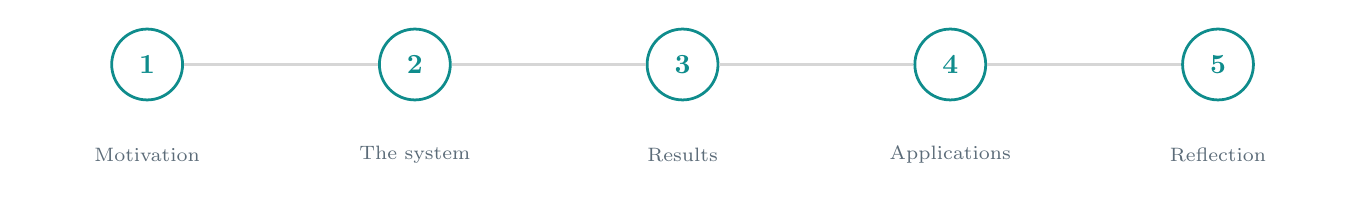
\begin{tikzpicture}[stn/.style={circle,draw=owteal,line width=1pt,minimum size=9mm,font=\bfseries,inner sep=0,text=owteal},std/.style={circle,draw=owteal,fill=owteal,line width=1pt,minimum size=9mm,font=\bfseries,inner sep=0,text=white},stc/.style={circle,draw=owochre,fill=owochre,line width=1.2pt,minimum size=11.5mm,font=\bfseries,inner sep=0,text=white},stx/.style={circle,draw=owmuted,line width=1pt,minimum size=9mm,font=\bfseries,inner sep=0,text=owmuted},stlbl/.style={font=\scriptsize,text=owmuted,align=center,text width=28mm},stln/.style={draw=black!16,line width=1.4pt}]\node[stn] (s0) at (0.0,0) {1};\node[stn] (s1) at (3.4,0) {2};\node[stn] (s2) at (6.8,0) {3};\node[stn] (s3) at (10.2,0) {4};\node[stn] (s4) at (13.6,0) {5};\node[stlbl] at (0.0,-1.15) {Motivation};\node[stlbl] at (3.4,-1.15) {The system};\node[stlbl] at (6.8,-1.15) {Results};\node[stlbl] at (10.2,-1.15) {Applications};\node[stlbl] at (13.6,-1.15) {Reflection};\draw[stln] (s0)--(s1);\draw[stln] (s1)--(s2);\draw[stln] (s2)--(s3);\draw[stln] (s3)--(s4);\end{tikzpicture}}\vfill\end{frame}
\begin{frame}[plain]\vfill\centering \resizebox{0.95\textwidth}{!}{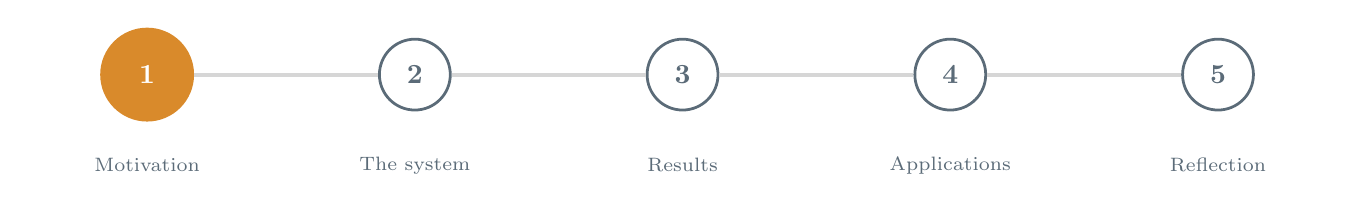
\begin{tikzpicture}[stn/.style={circle,draw=owteal,line width=1pt,minimum size=9mm,font=\bfseries,inner sep=0,text=owteal},std/.style={circle,draw=owteal,fill=owteal,line width=1pt,minimum size=9mm,font=\bfseries,inner sep=0,text=white},stc/.style={circle,draw=owochre,fill=owochre,line width=1.2pt,minimum size=11.5mm,font=\bfseries,inner sep=0,text=white},stx/.style={circle,draw=owmuted,line width=1pt,minimum size=9mm,font=\bfseries,inner sep=0,text=owmuted},stlbl/.style={font=\scriptsize,text=owmuted,align=center,text width=28mm},stln/.style={draw=black!16,line width=1.4pt}]\node[stc] (s0) at (0.0,0) {1};\node[stx] (s1) at (3.4,0) {2};\node[stx] (s2) at (6.8,0) {3};\node[stx] (s3) at (10.2,0) {4};\node[stx] (s4) at (13.6,0) {5};\node[stlbl] at (0.0,-1.15) {Motivation};\node[stlbl] at (3.4,-1.15) {The system};\node[stlbl] at (6.8,-1.15) {Results};\node[stlbl] at (10.2,-1.15) {Applications};\node[stlbl] at (13.6,-1.15) {Reflection};\draw[stln] (s0)--(s1);\draw[stln] (s1)--(s2);\draw[stln] (s2)--(s3);\draw[stln] (s3)--(s4);\end{tikzpicture}}\\[24pt]
{\color{owochre}\bfseries\footnotesize PART 1}\\[5pt]
{\color{owdeep}\bfseries\Large Motivation}\\[10pt]{\color{owmuted}\large From computing to world computing}\vfill\end{frame}
\begin{frame}{Prototyping a verified world}\vfill\begin{columns}[c]\begin{column}{0.323\textwidth}\centering{\color{owdeep}\fontsize{40}{44}\selectfont\bfseries 100}\\[6pt]{\color{owmuted}\small world models, 6 sectors}\end{column}\begin{column}{0.323\textwidth}\centering{\color{owochre}\fontsize{40}{44}\selectfont\bfseries 2.8 min}\\[6pt]{\color{owmuted}\small median build time}\end{column}\begin{column}{0.323\textwidth}\centering{\color{owdeep}\fontsize{40}{44}\selectfont\bfseries 47,000×}\\[6pt]{\color{owmuted}\small faster than an LLM}\end{column}\end{columns}\vfill\end{frame}
\begin{frame}{What is a world computer?}
\begin{itemize}
  \item Hardware + software that instantiates, verifies, composes, runs simulated worlds
  \item Dynamics are executable, checkable code -- not learned weights
  \item Classical computing made computation a cheap, inspectable commodity
  \item World computing aims to do the same for worlds
  \item Unit of work: a world model -- predicts next state given state and action
\end{itemize}
\end{frame}
\begin{frame}{Two species of world models}\vfill
\begin{columns}[T]
\begin{column}{0.46\textwidth}{\color{owmuted}\bfseries\large Perceptual / generative}\par\medskip\begin{itemize}\small \item Pixels / latents (Dreamer, Sora)
\item Data-hungry
\item Compounding error
\item Opaque weights\end{itemize}\end{column}
\begin{column}{0.46\textwidth}{\color{owteal}\bfseries\large Code world models}\par\medskip\begin{itemize}\small \item A readable program over state
\item Synthesized, then verified
\item Exact at every depth
\item Auditable source\end{itemize}\end{column}
\end{columns}\vfill\end{frame}
\begin{frame}{Why verified code}
\begin{itemize}
  \item Value is not novel dynamics -- the model can often recite the rule
  \item It is exact, fast, auditable execution an agent can call as a tool
  \item Deterministic: no compounding error; learned dynamics decay as (1-e)\textasciicircum{}t
  \item Plain code rolls out orders of magnitude faster than a per-step LLM
  \item PyTorch didn't give new models -- it made them fast to prototype
\end{itemize}
\end{frame}
\begin{frame}{World, action, agent, simulation}
\begin{itemize}
  \item World = symbolic state + discrete actions + verified transition
  \item Agent = a separate policy; a user of a world, not part of it
  \item Simulation = agents in a world producing scored trajectories
  \item A verified model relocates the sim-to-real gap into spec + perception
  \item So one World serves as both ground-truth environment and planning model
\end{itemize}
\end{frame}
\begin{frame}{The world computer, benchmarked on cost, latency, performance}
\centering

\includegraphics[width=\linewidth,height=0.48\textheight,keepaspectratio]{world_computer.png}\vskip3pt{\color{owmuted}\footnotesize One agent authors validated, servable worlds; verified code rolls out \textasciitilde{}47,000x faster than an LLM\par}
\flushleft \vskip3pt{\footnotesize \begin{itemize}
  \item A: 100 worlds authored at a median of 2.8 min each (p90 3.9)
  \item B: verified code at 14,997 steps/s vs 0.32 for a per-step LLM proxy
  \item C: 100\% validate structurally, 99\% pass a behavioral execution audit
\end{itemize}}
\end{frame}
\begin{frame}{Contributions}
\begin{itemize}
  \item World computing + a verification-preserving composition algebra
  \item OpenWorld: declared worlds, verified code, dial-steerable objectives
  \item Prototyping: 100 worlds, 6 sectors, minutes each, on consumer hardware
  \item Runtime: native-speed, exact, inspectable rollouts
  \item Evaluation, trust gates, and portable, auditable specs
\end{itemize}
\end{frame}
\begin{frame}[plain]\vfill\centering \resizebox{0.95\textwidth}{!}{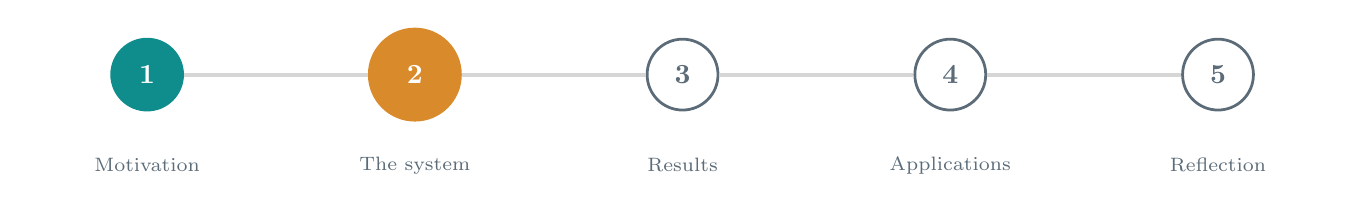
\begin{tikzpicture}[stn/.style={circle,draw=owteal,line width=1pt,minimum size=9mm,font=\bfseries,inner sep=0,text=owteal},std/.style={circle,draw=owteal,fill=owteal,line width=1pt,minimum size=9mm,font=\bfseries,inner sep=0,text=white},stc/.style={circle,draw=owochre,fill=owochre,line width=1.2pt,minimum size=11.5mm,font=\bfseries,inner sep=0,text=white},stx/.style={circle,draw=owmuted,line width=1pt,minimum size=9mm,font=\bfseries,inner sep=0,text=owmuted},stlbl/.style={font=\scriptsize,text=owmuted,align=center,text width=28mm},stln/.style={draw=black!16,line width=1.4pt}]\node[std] (s0) at (0.0,0) {1};\node[stc] (s1) at (3.4,0) {2};\node[stx] (s2) at (6.8,0) {3};\node[stx] (s3) at (10.2,0) {4};\node[stx] (s4) at (13.6,0) {5};\node[stlbl] at (0.0,-1.15) {Motivation};\node[stlbl] at (3.4,-1.15) {The system};\node[stlbl] at (6.8,-1.15) {Results};\node[stlbl] at (10.2,-1.15) {Applications};\node[stlbl] at (13.6,-1.15) {Reflection};\draw[stln] (s0)--(s1);\draw[stln] (s1)--(s2);\draw[stln] (s2)--(s3);\draw[stln] (s3)--(s4);\end{tikzpicture}}\\[24pt]
{\color{owochre}\bfseries\footnotesize PART 2}\\[5pt]
{\color{owdeep}\bfseries\Large The system}\\[10pt]{\color{owmuted}\large OpenWorld: components, the relay, composition}\vfill\end{frame}
\begin{frame}{Six unit-testable components}
\begin{itemize}
  \item World: state ontology, actions, rules, pluggable transition engine
  \item Three engines: CodeTransition, LLMTransition (baseline), FunctionTransition (oracle)
  \item Agent: LLM planner or deterministic policy
  \item Objective + Dial: open, tunable value specification
  \item Simulation, Tuner, Judge -- all over a local Ollama backbone, zero runtime deps
\end{itemize}
\end{frame}
\begin{frame}{The plan--generate--verify relay}\vfill\centering
\resizebox{0.98\textwidth}{!}{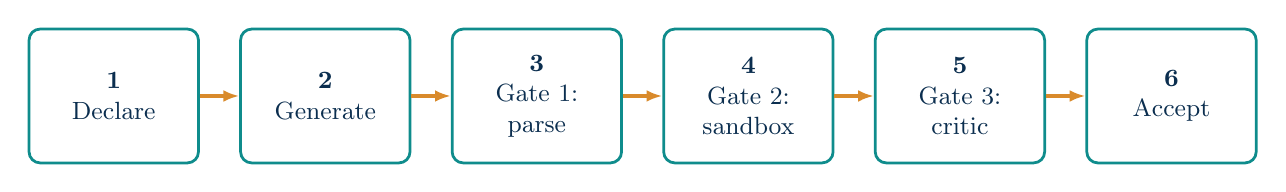
\begin{tikzpicture}[node distance=5mm and 5mm,
  sb/.style={draw=owteal,line width=1pt,rounded corners=4pt,fill=white,inner sep=5pt,
  text width=18mm,align=center,minimum height=17mm,font=\small,text=owdeep}]
\node[sb] (n0) {\textbf{1}\\ Declare};\node[sb,right=of n0] (n1) {\textbf{2}\\ Generate};\node[sb,right=of n1] (n2) {\textbf{3}\\ Gate 1: parse};\node[sb,right=of n2] (n3) {\textbf{4}\\ Gate 2: sandbox};\node[sb,right=of n3] (n4) {\textbf{5}\\ Gate 3: critic};\node[sb,right=of n4] (n5) {\textbf{6}\\ Accept};
\draw[-{Latex[length=2mm]},owochre,line width=1.1pt] (n0) -- (n1);\draw[-{Latex[length=2mm]},owochre,line width=1.1pt] (n1) -- (n2);\draw[-{Latex[length=2mm]},owochre,line width=1.1pt] (n2) -- (n3);\draw[-{Latex[length=2mm]},owochre,line width=1.1pt] (n3) -- (n4);\draw[-{Latex[length=2mm]},owochre,line width=1.1pt] (n4) -- (n5);
\end{tikzpicture}}\vfill\end{frame}
\begin{frame}{A code world model, end to end}
\centering

\includegraphics[width=\linewidth,height=0.48\textheight,keepaspectratio]{prototyping_pipeline.png}\vskip3pt{\color{owmuted}\footnotesize Perceive -> world -> emit/act, generated from a real spec so labels cannot drift\par}
\flushleft \vskip3pt{\footnotesize \begin{itemize}
  \item Perceptors turn any-modality inputs into symbolic state
  \item Verified transitions step inside a composite of nested worlds
  \item Objectives (dial-retuned) score; emit/act boundary returns reports and tool-calls
\end{itemize}}
\end{frame}
\begin{frame}{A composition algebra for worlds}
\begin{itemize}
  \item Worlds are values; compose() is closed -- output is itself a world
  \item Children run unmodified; bridges couple, aggregators roll up, bindings inject
  \item Closure, identity, and associativity hold up to namespace renaming
  \item Verification is compositional: verified pieces => verified whole
  \item Turns one n-rule synthesis into n small, independently verified problems
\end{itemize}
\end{frame}
\begin{frame}{Verified reward induction}
\begin{itemize}
  \item Objective made symmetric to the transition: a verified reward as code
  \item CodeObjective's reward() runs in the same pure-Python sandbox
  \item induce\_reward accepts only when it exact-matches held-out rewards
  \item Closes the loop: verified perception + dynamics + reward + planning
  \item The primitive ARC-AGI-3-style goal discovery demands
\end{itemize}
\end{frame}
\begin{frame}[plain]\centering\vfill
{\color{owochre}\rule{40pt}{2.5pt}}\par\vskip10pt
{\color{owdeep}\bfseries\Large Prototyping cost \& latency\par}\vfill\end{frame}
\begin{frame}{How fast is prototyping? (E68)}
\begin{itemize}
  \item Claude Code authored 100 world models from one-line descriptions
  \item 6 regulated sectors: health, finance, legal, cyber, energy, agentic-AI
  \item 100\% validate; median 2.8 min, mean 3.0, p90 3.9, max 6.1
  \item 99\% (99/100) are behaviorally executable under a random rollout
  \item Hand-authoring a comparable simulator is a days-to-weeks effort
\end{itemize}
\end{frame}
\begin{frame}{Atlas of the 100 prototyped worlds (E68/E68b)}
\centering
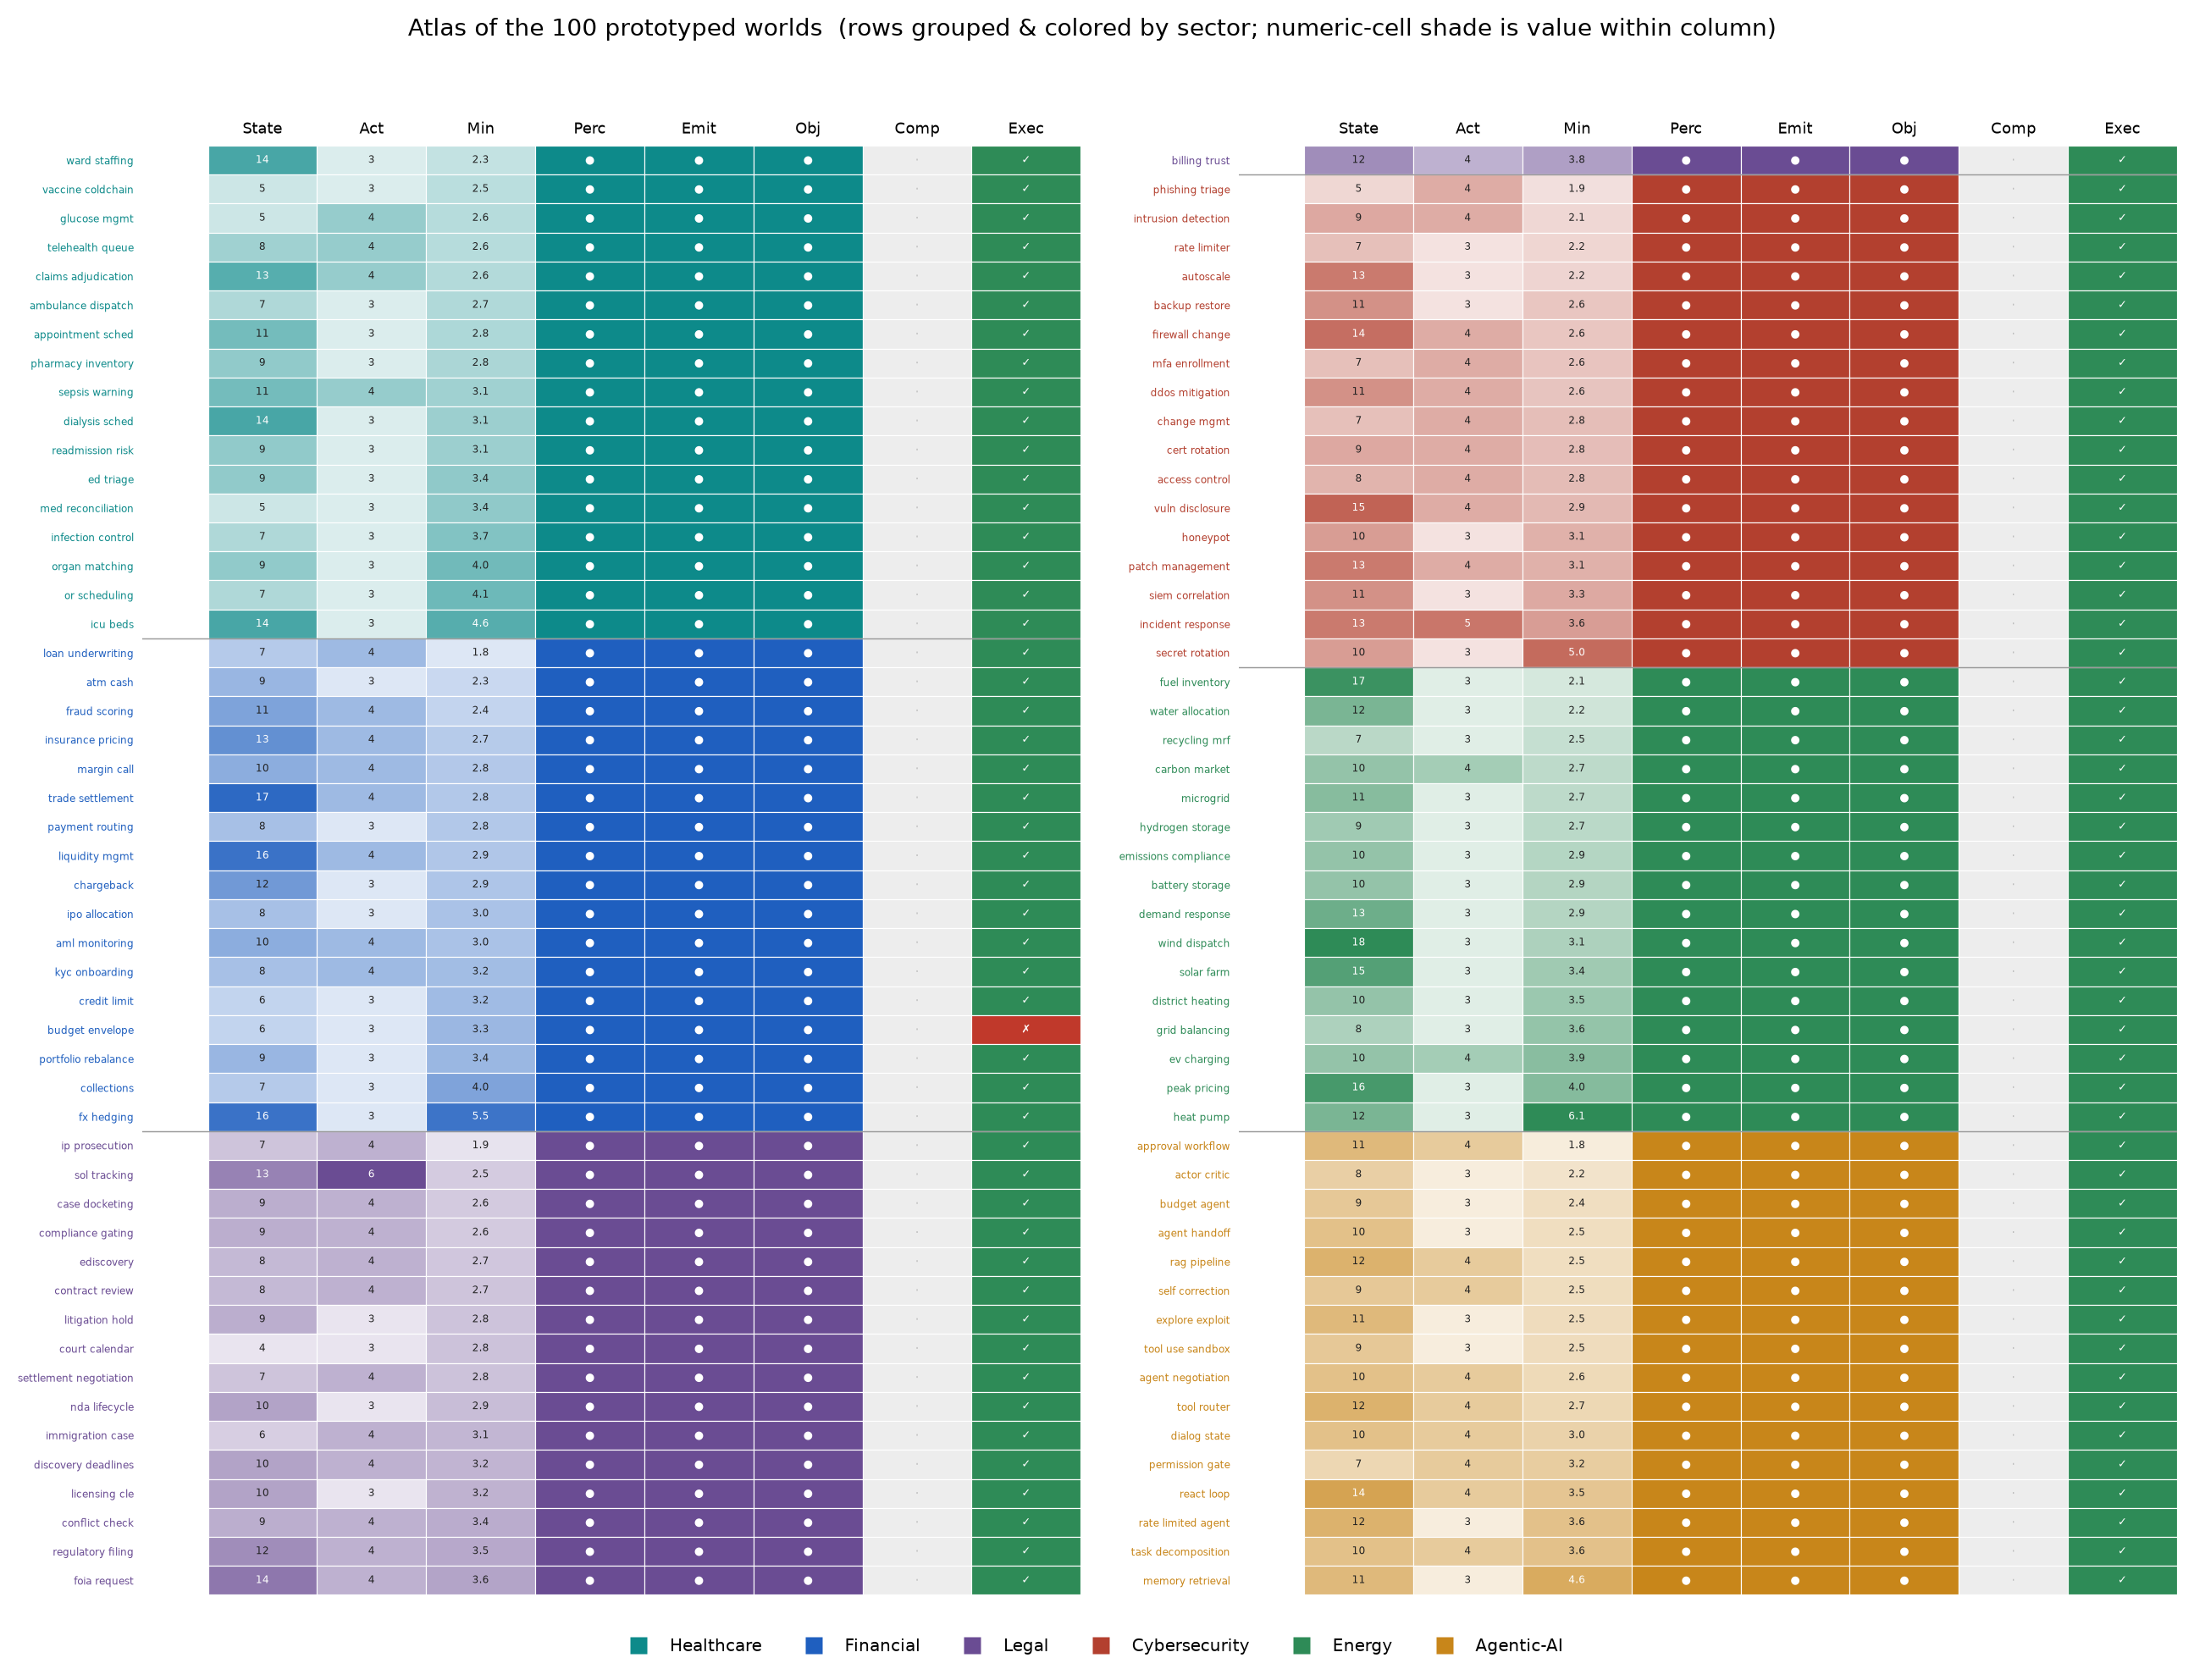
\includegraphics[width=\linewidth,height=0.48\textheight,keepaspectratio]{world_atlas.png}\vskip3pt{\color{owmuted}\footnotesize One row per world, grouped by sector; all declare perceive and emit boundaries\par}
\flushleft \vskip3pt{\footnotesize \begin{itemize}
  \item Columns: state size, actions, build minutes, declared boundaries
  \item Exec marks the behavioral audit -- only one recipe fails to evolve state
  \item Generated from per-world records, so it cannot drift from results
\end{itemize}}
\end{frame}
\begin{frame}[plain]\centering\vfill
{\color{owdeep}\bfseries\LARGE When dynamics are writable, prototyping a correct world model is a minutes-scale, push-button activity.\par}\vfill\end{frame}
\begin{frame}[plain]\centering\vfill
{\color{owochre}\rule{40pt}{2.5pt}}\par\vskip10pt
{\color{owdeep}\bfseries\Large Experimental setup\par}\vfill\end{frame}
\begin{frame}{Worlds with ground truth}
\begin{itemize}
  \item Three deterministic oracle worlds: sprint, orchard, triage
  \item Oracles are hand-written FunctionTransitions
  \item Synthesized and learned engines compared against them exactly
  \item Coding world: 20 buggy functions + hidden tests, test-execution dynamics
  \item Composition/nesting/changing-rules probed by E30--E32
\end{itemize}
\end{frame}
\begin{frame}{Models, hardware, baselines, statistics}
\begin{itemize}
  \item All local via Ollama on an Apple-silicon laptop -- no cloud, no fine-tuning
  \item qwen2.5 7b/3b/1.5b, plus llama3.1:8b and gemma2:9b for cross-family
  \item Baseline: LLMTransition -- same backbone predicting each next state
  \item Rate metrics get 95\% Wilson CIs; judge test is exact paired McNemar
  \item Seeds fixed; every number regenerates from one pipeline
\end{itemize}
\end{frame}
\begin{frame}[plain]\vfill\centering \resizebox{0.95\textwidth}{!}{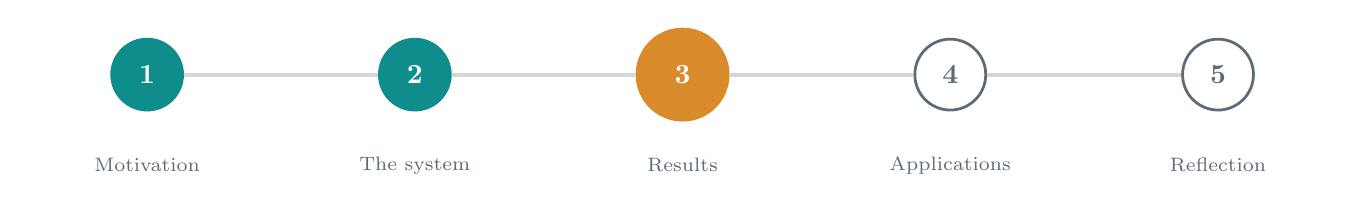
\begin{tikzpicture}[stn/.style={circle,draw=owteal,line width=1pt,minimum size=9mm,font=\bfseries,inner sep=0,text=owteal},std/.style={circle,draw=owteal,fill=owteal,line width=1pt,minimum size=9mm,font=\bfseries,inner sep=0,text=white},stc/.style={circle,draw=owochre,fill=owochre,line width=1.2pt,minimum size=11.5mm,font=\bfseries,inner sep=0,text=white},stx/.style={circle,draw=owmuted,line width=1pt,minimum size=9mm,font=\bfseries,inner sep=0,text=owmuted},stlbl/.style={font=\scriptsize,text=owmuted,align=center,text width=28mm},stln/.style={draw=black!16,line width=1.4pt}]\node[std] (s0) at (0.0,0) {1};\node[std] (s1) at (3.4,0) {2};\node[stc] (s2) at (6.8,0) {3};\node[stx] (s3) at (10.2,0) {4};\node[stx] (s4) at (13.6,0) {5};\node[stlbl] at (0.0,-1.15) {Motivation};\node[stlbl] at (3.4,-1.15) {The system};\node[stlbl] at (6.8,-1.15) {Results};\node[stlbl] at (10.2,-1.15) {Applications};\node[stlbl] at (13.6,-1.15) {Reflection};\draw[stln] (s0)--(s1);\draw[stln] (s1)--(s2);\draw[stln] (s2)--(s3);\draw[stln] (s3)--(s4);\end{tikzpicture}}\\[24pt]
{\color{owochre}\bfseries\footnotesize PART 3}\\[5pt]
{\color{owdeep}\bfseries\Large Results}\\[10pt]{\color{owmuted}\large Fidelity, latency, and trust}\vfill\end{frame}
\begin{frame}{Performance: fidelity and latency (E04, E11)}
\centering
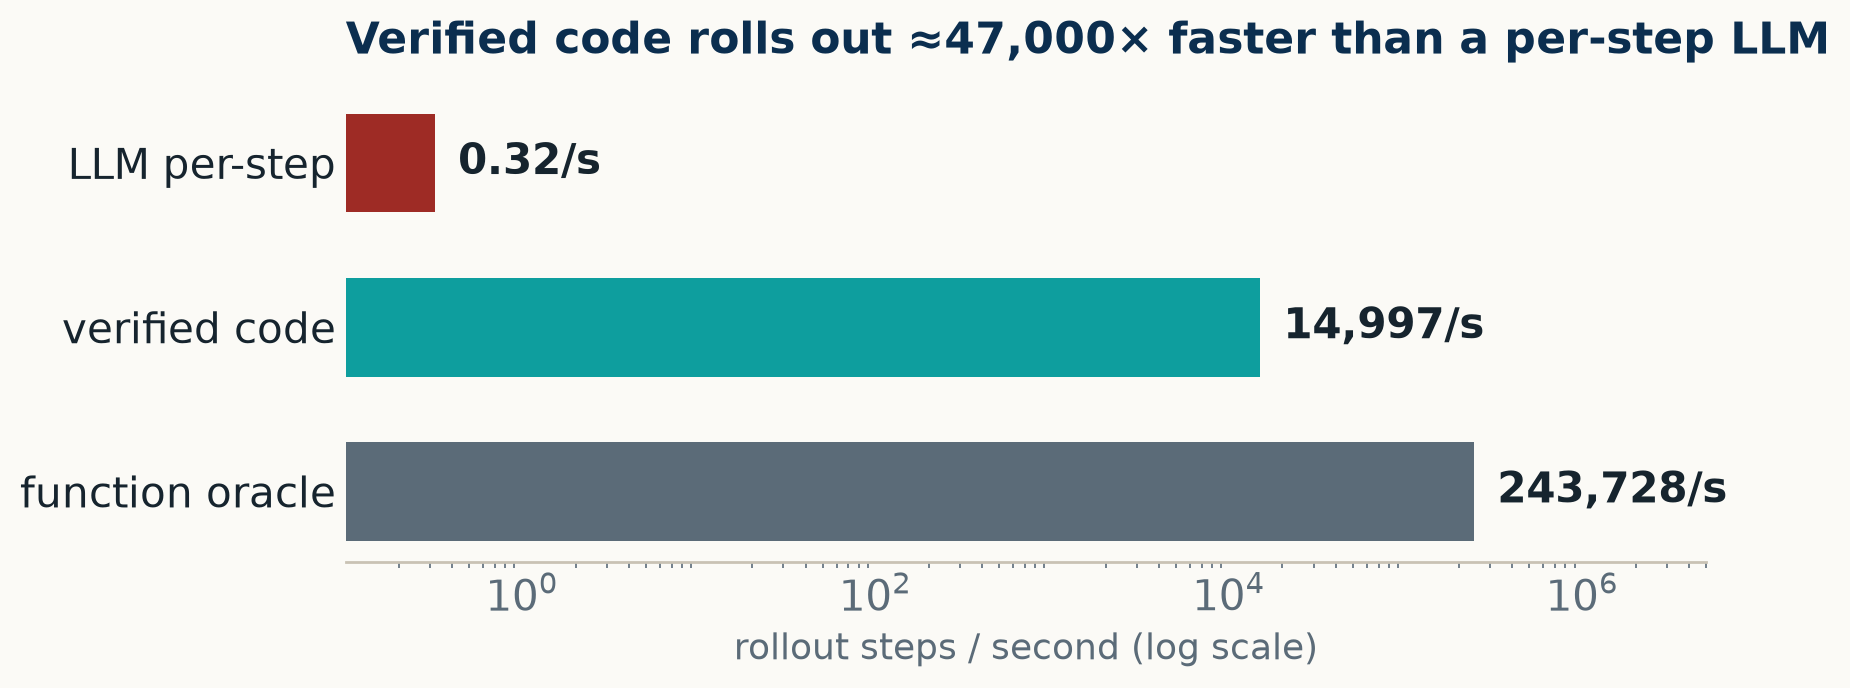
\includegraphics[width=\linewidth,height=0.48\textheight,keepaspectratio]{pres_speed.png}\vskip3pt{\color{owmuted}\footnotesize One verified transition reused at every step -- no compounding error\par}
\flushleft \vskip3pt{\footnotesize \begin{itemize}
  \item 7B-synthesized dynamics exact on 24/24 20-step rollouts; 100\% on 10x OOD probes
  \item 14,997 steps/s vs 0.32 for the LLM proxy (\textasciitilde{}47,000x)
\end{itemize}}
\end{frame}
\begin{frame}{Verifier ablation: correctness gained per gate (E3)}
\centering
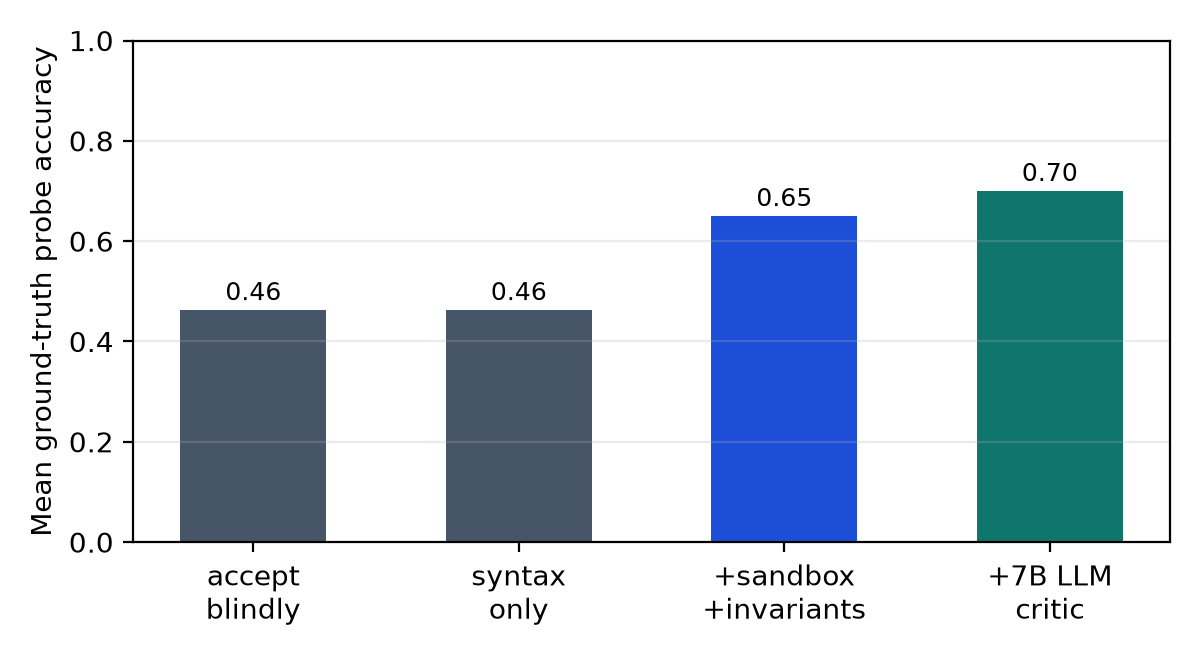
\includegraphics[width=\linewidth,height=0.48\textheight,keepaspectratio]{verifier.png}\vskip3pt{\color{owmuted}\footnotesize Blind 0.46 -> behavioral 0.65 -> +critic 0.70 (a +0.24 absolute gain)\par}
\flushleft \vskip3pt{\footnotesize \begin{itemize}
  \item Syntax-only adds nothing -- this generator's failures parse fine
  \item No 3B generation is bit-exact under any regime
  \item Verification buys correctness margin but cannot replace generator capability
\end{itemize}}
\end{frame}
\begin{frame}{Closing the false-accept gap (E62)}
\begin{itemize}
  \item Single-state smoke-run has a blind spot: later-reached states
  \item On 3 faults clean initially, single-state gate false-accepts 100\%
  \item Re-running over branch-covering states drops false-accepts to 0\%
  \item Cross-family (E16): Qwen/Llama/Gemma all reach verified acceptance
  \item Gemma-2-9B is rule-perfect on every attempt; seconds per world
\end{itemize}
\end{frame}
\begin{frame}{Agents-as-a-judge, controlled (E13+E17)}
\centering
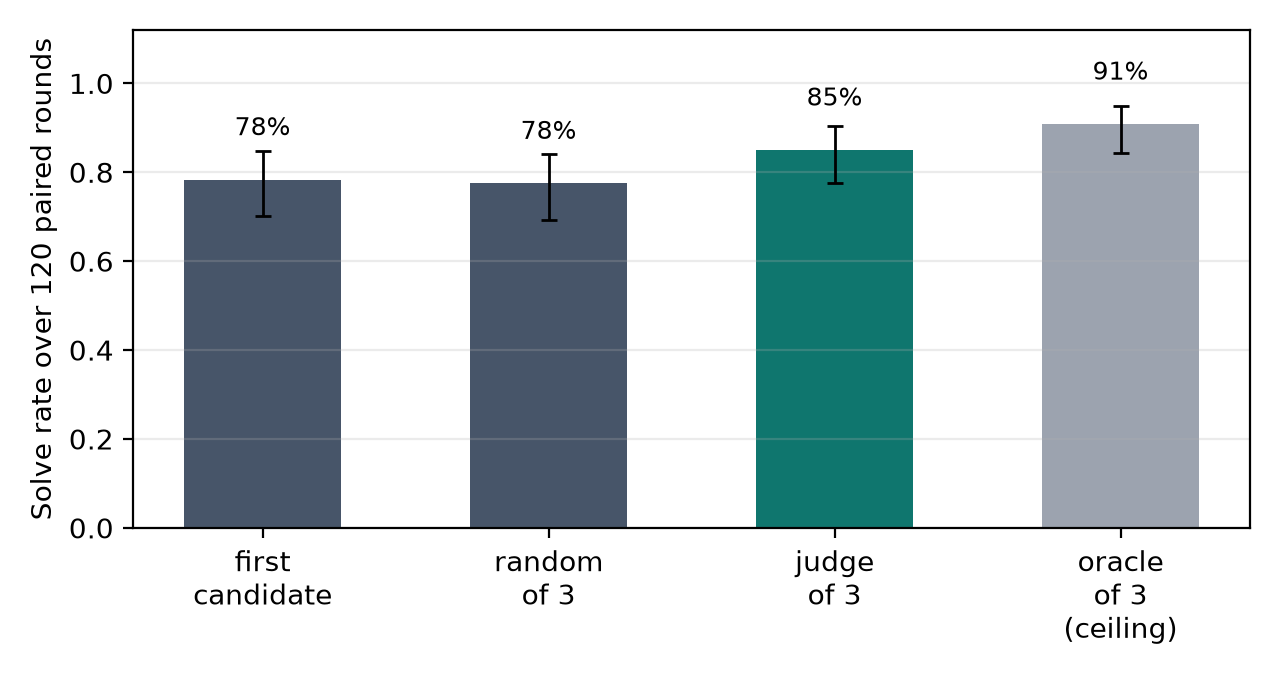
\includegraphics[width=\linewidth,height=0.48\textheight,keepaspectratio]{judge.png}\vskip3pt{\color{owmuted}\footnotesize Judge 85\% vs random 78\%, first 78\%, oracle ceiling 91\% over 120 rounds\par}
\flushleft \vskip3pt{\footnotesize \begin{itemize}
  \item Judge recovers \textasciitilde{}half the random-to-oracle gap (McNemar p marginal)
  \item Order-reversal: raw choices match \textasciitilde{}57\% but accuracy is order-stable
  \item Costs \textasciitilde{}4x inference; judges should gate, not replace, verification
\end{itemize}}
\end{frame}
\begin{frame}{Anatomy of a composite world (E31)}
\centering

\includegraphics[width=\linewidth,height=0.48\textheight,keepaspectratio]{composition.png}\vskip3pt{\color{owmuted}\footnotesize Two countries, each with two cities, compose into a region -- real state values\par}
\flushleft \vskip3pt{\footnotesize \begin{itemize}
  \item Bridge carries trade under a conservation invariant
  \item Route lets an agent cross and pay a toll; aggregators summarize upward
  \item Binding injects a parent parameter into a child
\end{itemize}}
\end{frame}
\begin{frame}{Composition defeats the complexity cliff (E30)}
\centering
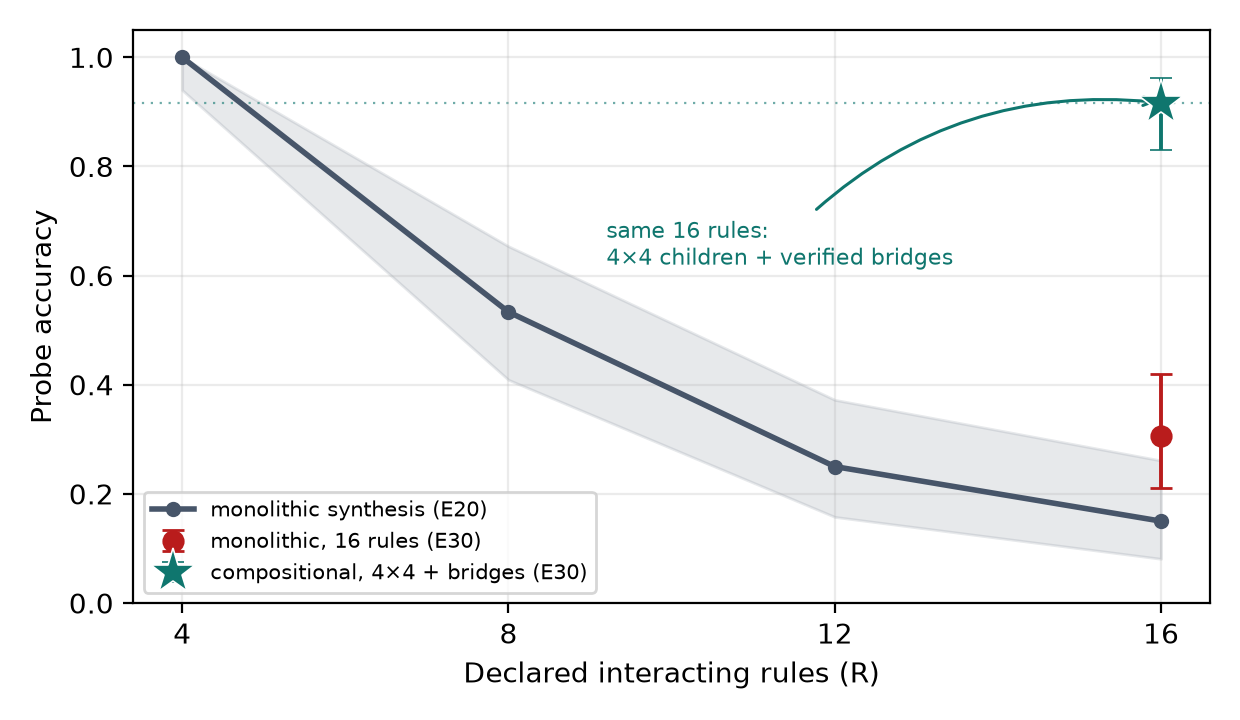
\includegraphics[width=\linewidth,height=0.48\textheight,keepaspectratio]{composition_cliff.png}\vskip3pt{\color{owmuted}\footnotesize 16 rules: monolithic 0.31 vs four 4-rule children + bridges 0.92\par}
\flushleft \vskip3pt{\footnotesize \begin{itemize}
  \item Monolithic 7B synthesis collapses past \textasciitilde{}8 coupled rules
  \item Decomposition returns accuracy to near-R=4 levels
  \item Acceptance identical in both conditions -- the decomposition is the difference
\end{itemize}}
\end{frame}
\begin{frame}{What an agent sees (E31)}
\centering
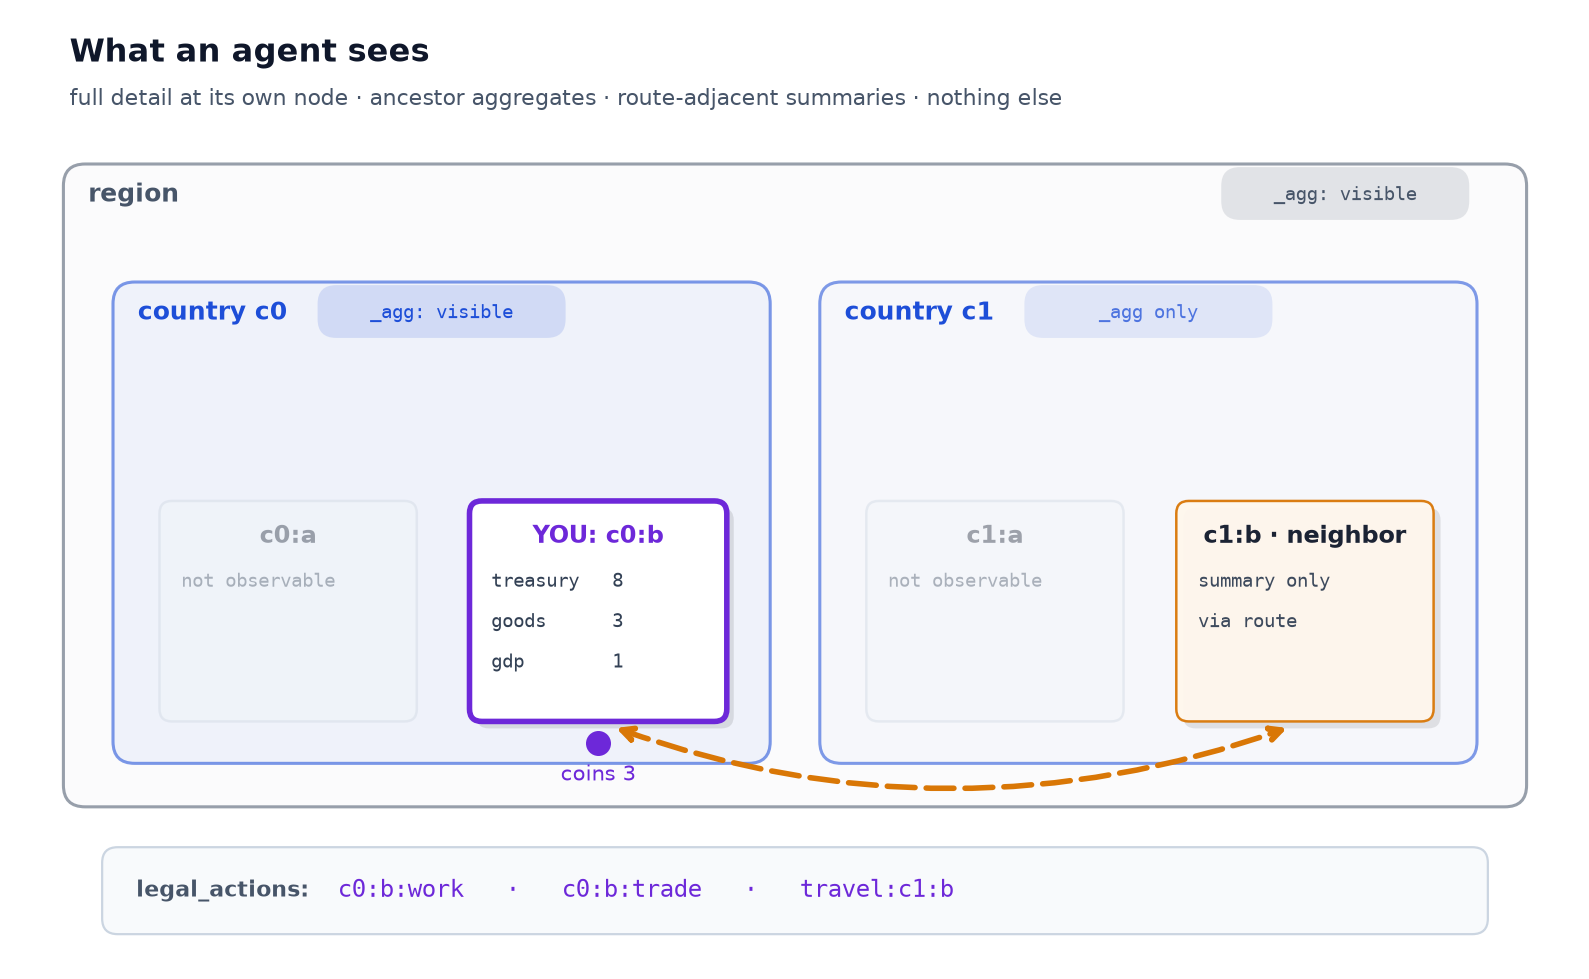
\includegraphics[width=\linewidth,height=0.48\textheight,keepaspectratio]{traversal.png}\vskip3pt{\color{owmuted}\footnotesize Scoped observation: own node full, ancestors as aggregates, neighbors as summaries\par}
\flushleft \vskip3pt{\footnotesize \begin{itemize}
  \item Its own city fully observable; ancestor levels expose only \_agg summaries
  \item Route-adjacent city is a summary card; siblings not observable
  \item Planners reason locally against exact dynamics without the macrostate
\end{itemize}}
\end{frame}
\begin{frame}{When the rules change, agents move (E33)}
\centering
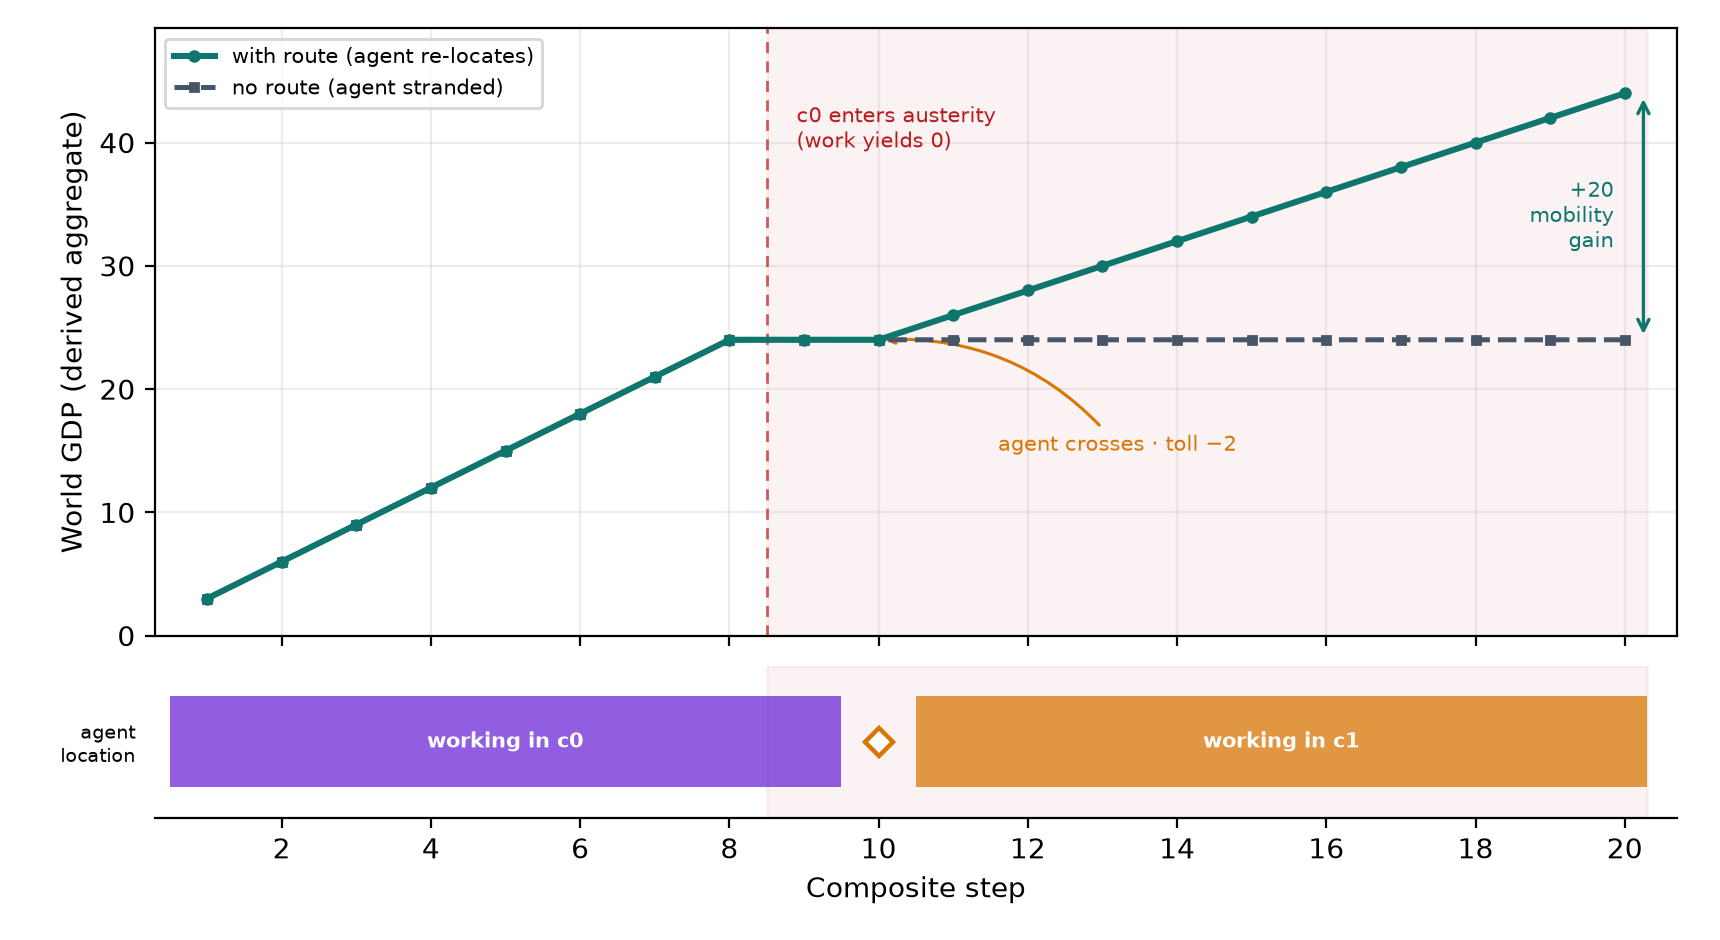
\includegraphics[width=\linewidth,height=0.48\textheight,keepaspectratio]{dynamic_traversal.png}\vskip3pt{\color{owmuted}\footnotesize Austerity hits at step 9; agent pays the toll, relocates, gains +20 mobility\par}
\flushleft \vskip3pt{\footnotesize \begin{itemize}
  \item Shared economy enters austerity via PhasedTransition
  \item Greedy agent prices the change and crosses to the growing economy
  \item Both phased and monolithic synthesized code track the switch exactly
\end{itemize}}
\end{frame}
\begin{frame}{The sprint world: budget allocation (E34)}
\centering

\includegraphics[width=\linewidth,height=0.48\textheight,keepaspectratio]{sprint.png}\vskip3pt{\color{owmuted}\footnotesize 20 repair worlds, budget 80; fixed protocol solves 15/20\par}
\flushleft \vskip3pt{\footnotesize \begin{itemize}
  \item No policy beats the fixed ceiling -- the unsolved tail is capability-bound
  \item Round-robin reaches the plateau in \textasciitilde{}a third fewer attempts
  \item Greedy closest-to-passing tarpits on a single task
\end{itemize}}
\end{frame}
\begin{frame}{Perceive-then-forecast an SIR epidemic (E40)}
\centering

\includegraphics[width=\linewidth,height=0.48\textheight,keepaspectratio]{perception.png}\vskip3pt{\color{owmuted}\footnotesize Perceived world model is exact in and out of distribution; the MLP collapses at 10x scale\par}
\flushleft \vskip3pt{\footnotesize \begin{itemize}
  \item Day-0 text + ward-photo perceived into S,I,R, then rolled 14 days
  \item Dynamics add zero error, so forecast accuracy equals perception accuracy
  \item E39: this decomposition holds exactly across perception error 0--0.9
\end{itemize}}
\end{frame}
\begin{frame}{Tunable morality: the moral dial (E8)}
\centering

\includegraphics[width=\linewidth,height=0.48\textheight,keepaspectratio]{pareto.png}\vskip3pt{\color{owmuted}\footnotesize Welfare--fairness frontier swept by lambda; Nash bargaining optimum interior at 0.8\par}
\flushleft \vskip3pt{\footnotesize \begin{itemize}
  \item All 11 sweep points are Pareto-optimal; fairness monotone in lambda
  \item Values are declared, weighted artifacts -- no retraining to move
  \item Operationalizes the open-specification response to static alignment
\end{itemize}}
\end{frame}
\begin{frame}[plain]\centering\vfill
{\color{owochre}\rule{40pt}{2.5pt}}\par\vskip10pt
{\color{owdeep}\bfseries\Large Shareable, auditable worlds\par}\vfill\end{frame}
\begin{frame}{Portable world-model specs (E57)}
\centering
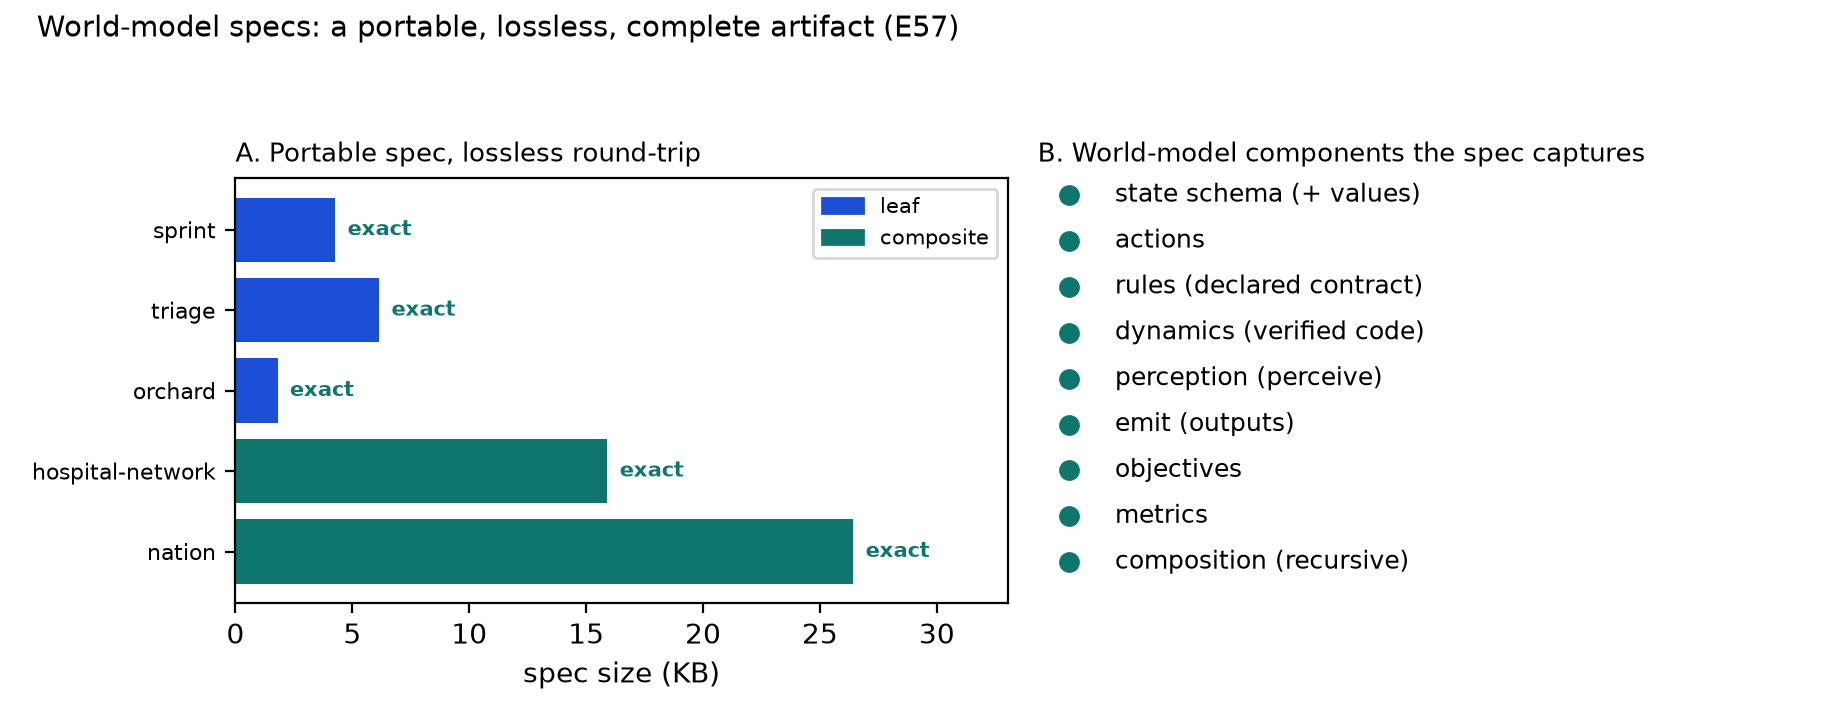
\includegraphics[width=\linewidth,height=0.48\textheight,keepaspectratio]{world_specs.png}\vskip3pt{\color{owmuted}\footnotesize 5 worlds round-trip losslessly at a few KB; nine components captured\par}
\flushleft \vskip3pt{\footnotesize \begin{itemize}
  \item from\_spec(to\_spec(w)) reproduces the original rollout exactly
  \item State, rules, dynamics, perception/emit, objectives, metrics -- all captured
  \item Embedded code is inert unless execution is explicitly opted in
\end{itemize}}
\end{frame}
\begin{frame}{A generated model card (E57)}
\centering
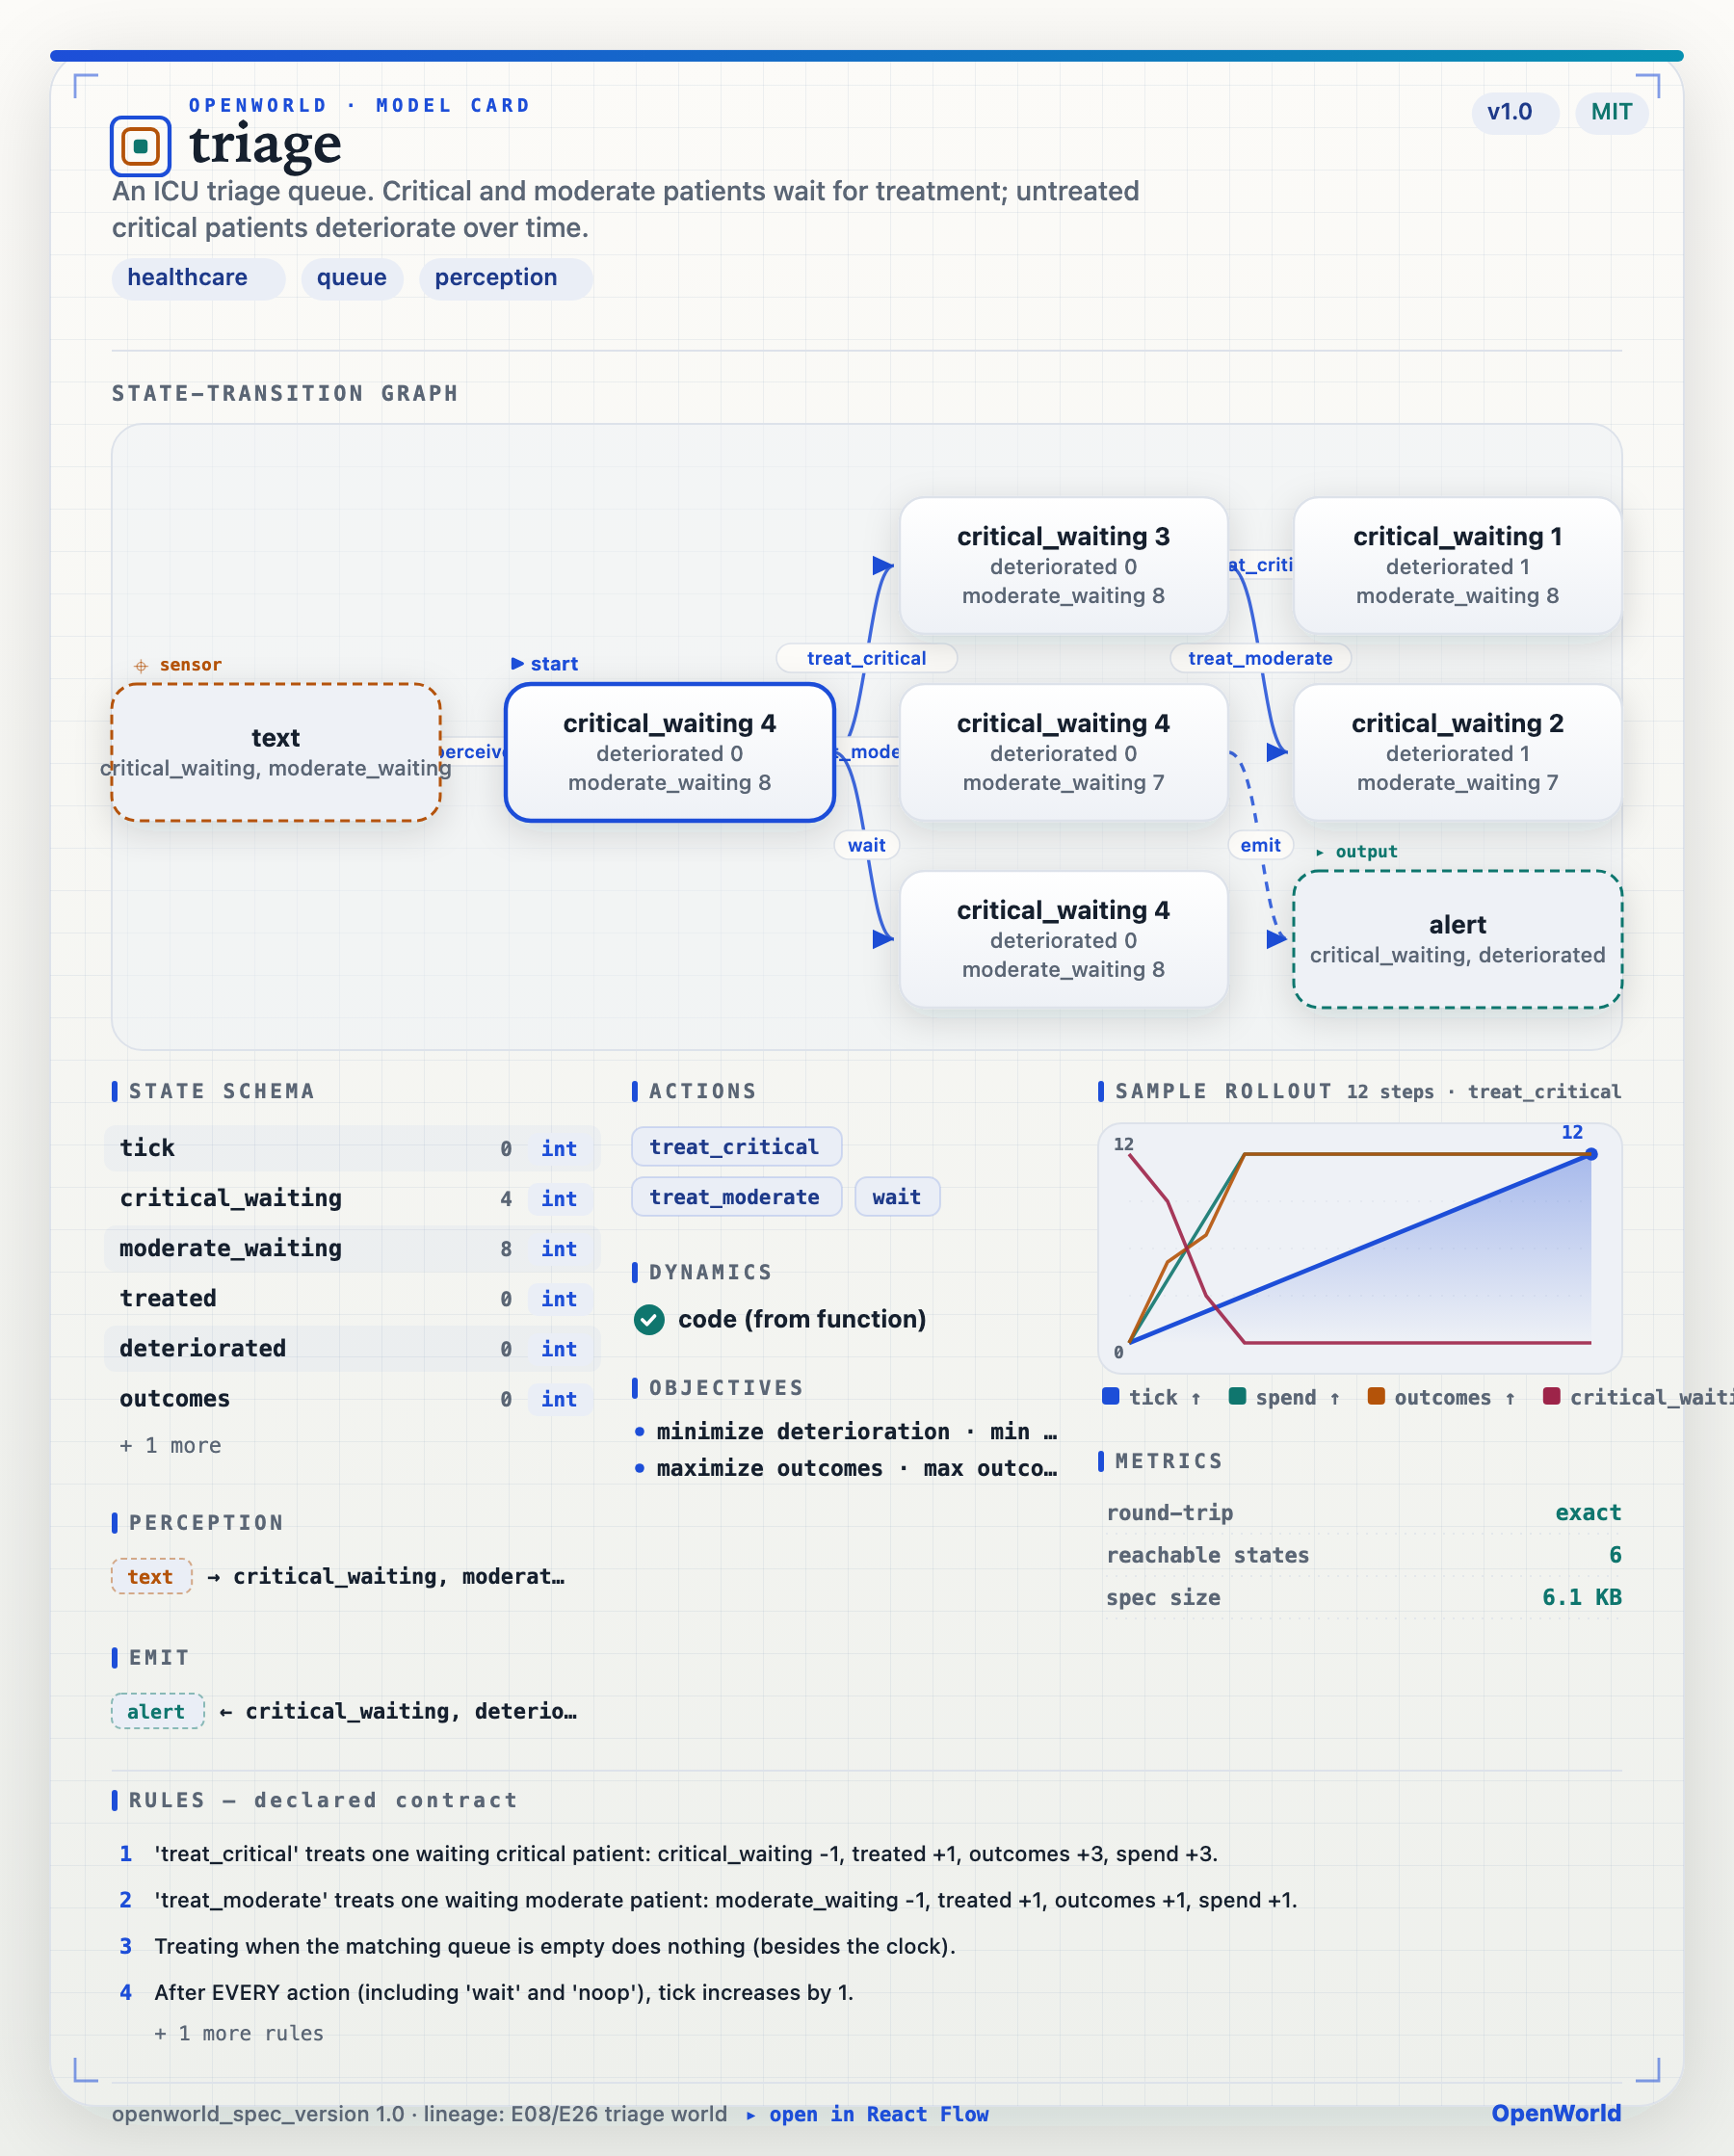
\includegraphics[width=\linewidth,height=0.48\textheight,keepaspectratio]{world_card.png}\vskip3pt{\color{owmuted}\footnotesize One self-contained SVG rendered from the triage world's spec\par}
\flushleft \vskip3pt{\footnotesize \begin{itemize}
  \item State-transition automaton with the perceive->world->emit boundary
  \item Panels list schema, actions, dynamics, objectives, rollout, metrics
  \item Also exports to Mermaid and React Flow for interactive use
\end{itemize}}
\end{frame}
\begin{frame}[plain]\vfill\centering \resizebox{0.95\textwidth}{!}{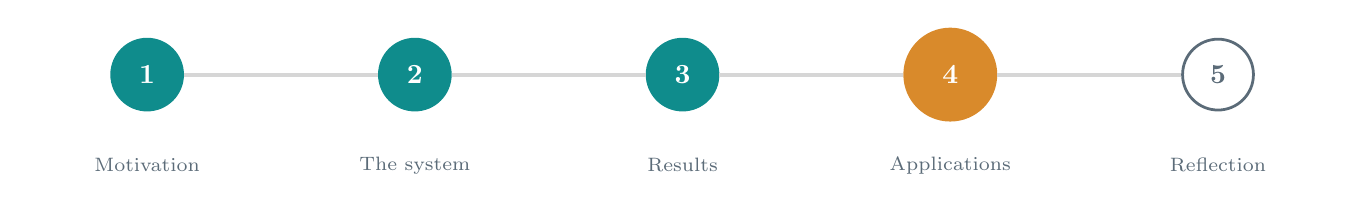
\begin{tikzpicture}[stn/.style={circle,draw=owteal,line width=1pt,minimum size=9mm,font=\bfseries,inner sep=0,text=owteal},std/.style={circle,draw=owteal,fill=owteal,line width=1pt,minimum size=9mm,font=\bfseries,inner sep=0,text=white},stc/.style={circle,draw=owochre,fill=owochre,line width=1.2pt,minimum size=11.5mm,font=\bfseries,inner sep=0,text=white},stx/.style={circle,draw=owmuted,line width=1pt,minimum size=9mm,font=\bfseries,inner sep=0,text=owmuted},stlbl/.style={font=\scriptsize,text=owmuted,align=center,text width=28mm},stln/.style={draw=black!16,line width=1.4pt}]\node[std] (s0) at (0.0,0) {1};\node[std] (s1) at (3.4,0) {2};\node[std] (s2) at (6.8,0) {3};\node[stc] (s3) at (10.2,0) {4};\node[stx] (s4) at (13.6,0) {5};\node[stlbl] at (0.0,-1.15) {Motivation};\node[stlbl] at (3.4,-1.15) {The system};\node[stlbl] at (6.8,-1.15) {Results};\node[stlbl] at (10.2,-1.15) {Applications};\node[stlbl] at (13.6,-1.15) {Reflection};\draw[stln] (s0)--(s1);\draw[stln] (s1)--(s2);\draw[stln] (s2)--(s3);\draw[stln] (s3)--(s4);\end{tikzpicture}}\\[24pt]
{\color{owochre}\bfseries\footnotesize PART 4}\\[5pt]
{\color{owdeep}\bfseries\Large Applications}\\[10pt]{\color{owmuted}\large Domains and demonstrations}\vfill\end{frame}
\begin{frame}{Emergent economy from composed verified rules (E44)}
\centering
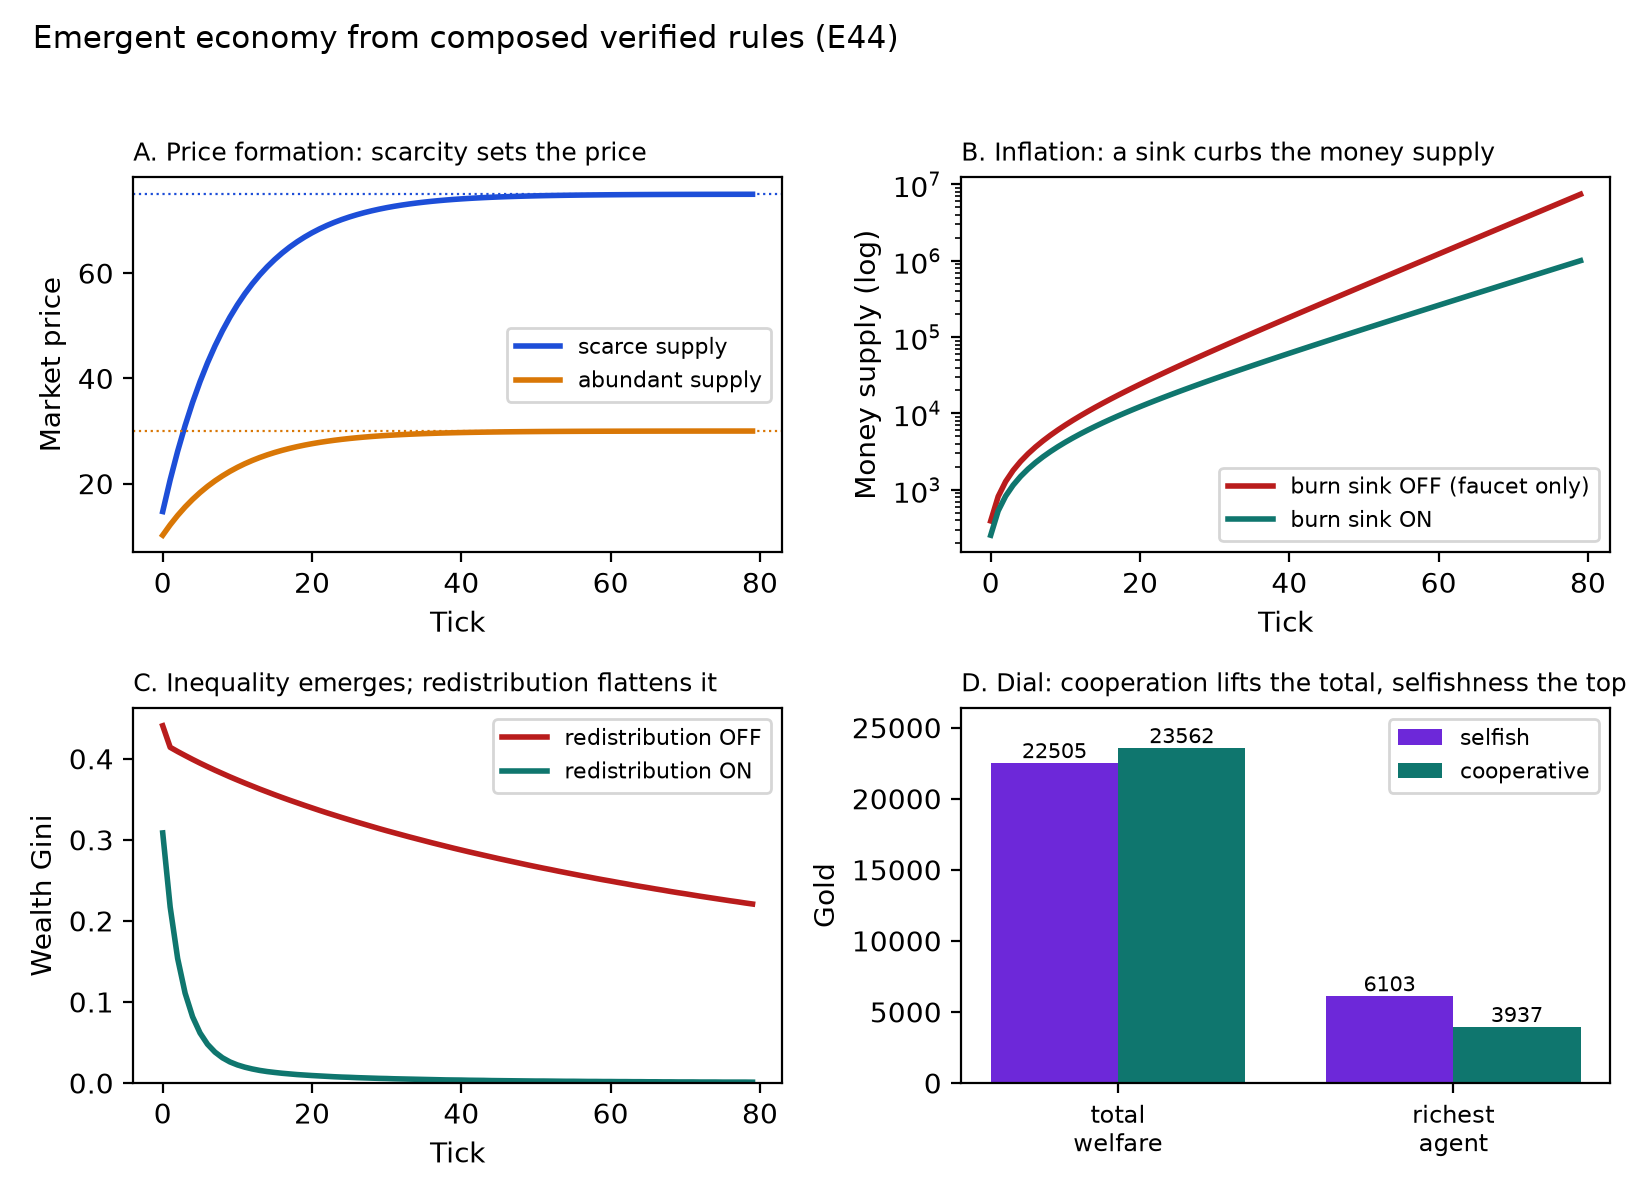
\includegraphics[width=\linewidth,height=0.48\textheight,keepaspectratio]{emergent_economy.png}\vskip3pt{\color{owmuted}\footnotesize 6 agents; Gini 0.22 -> 0.001 with redistribution; cooperation lifts welfare\par}
\flushleft \vskip3pt{\footnotesize \begin{itemize}
  \item Macro (price, inflation, Gini) are aggregators derived from micro leaves
  \item Each phenomenon isolated by toggling one verified rule
  \item Books balance exactly every tick -- gold moves only by faucet minus sink
\end{itemize}}
\end{frame}
\begin{frame}{A composite corporate world (E48)}
\centering

\includegraphics[width=\linewidth,height=0.48\textheight,keepaspectratio]{corporate_world.png}\vskip3pt{\color{owmuted}\footnotesize 5-division, \$1500M PaaS as nested CompositeWorld; CEO reallocation is +21\%\par}
\flushleft \vskip3pt{\footnotesize \begin{itemize}
  \item Company > divisions > individuals; revenue aggregates upward
  \item Selfishness trades company growth for a higher promotion Gini
  \item Perception is granularity-bound: promo signal recovered only from 1:1s
\end{itemize}}
\end{frame}
\begin{frame}{A startup growth world model (E51)}
\centering
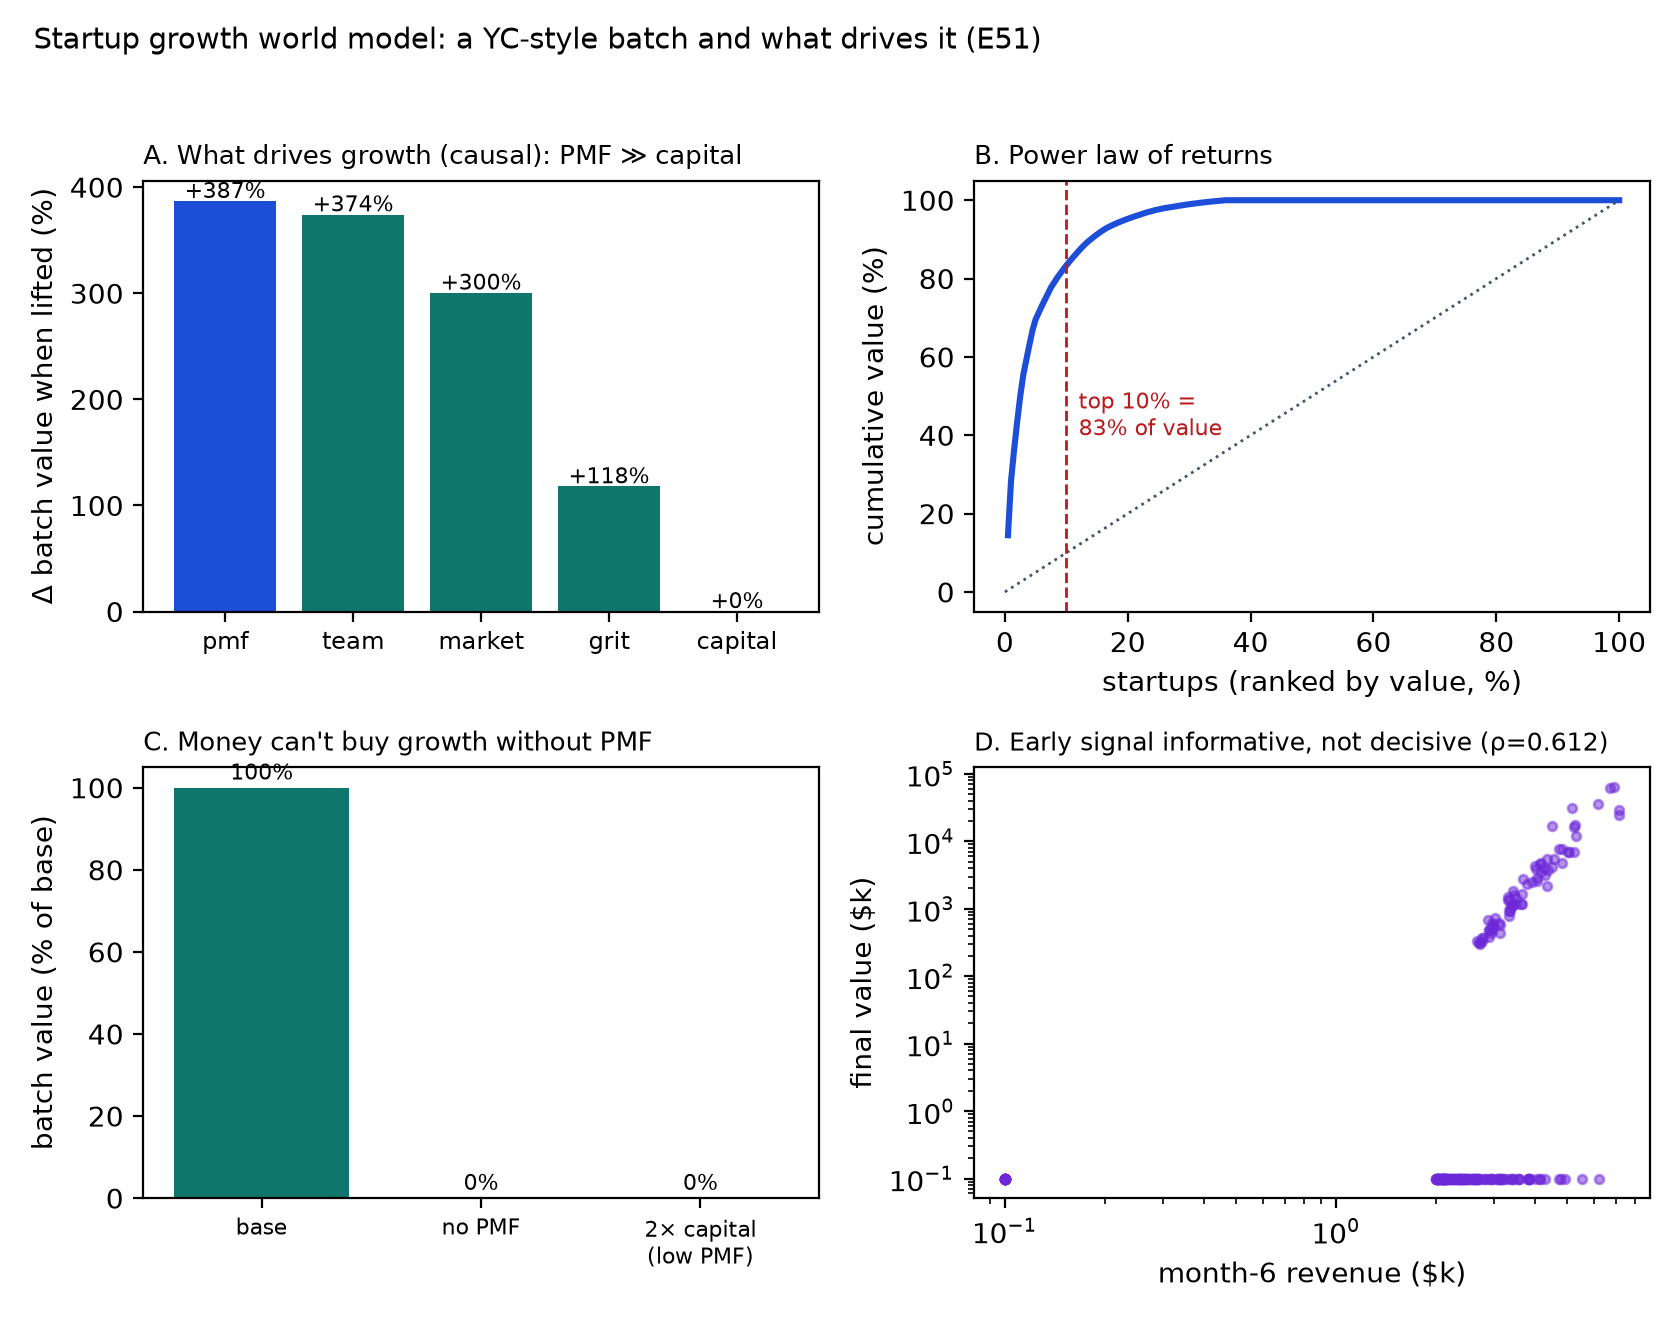
\includegraphics[width=\linewidth,height=0.48\textheight,keepaspectratio]{startups.png}\vskip3pt{\color{owmuted}\footnotesize PMF moves value +387\%; capital +0\%; top decile captures 83\% of value\par}
\flushleft \vskip3pt{\footnotesize \begin{itemize}
  \item Each startup a verified child world; batch aggregates exactly
  \item Only 36\% survive -- the venture power law reproduced
  \item Spend cannot substitute for product-market fit
\end{itemize}}
\end{frame}
\begin{frame}{Relativity as a verified world model (E47)}
\centering
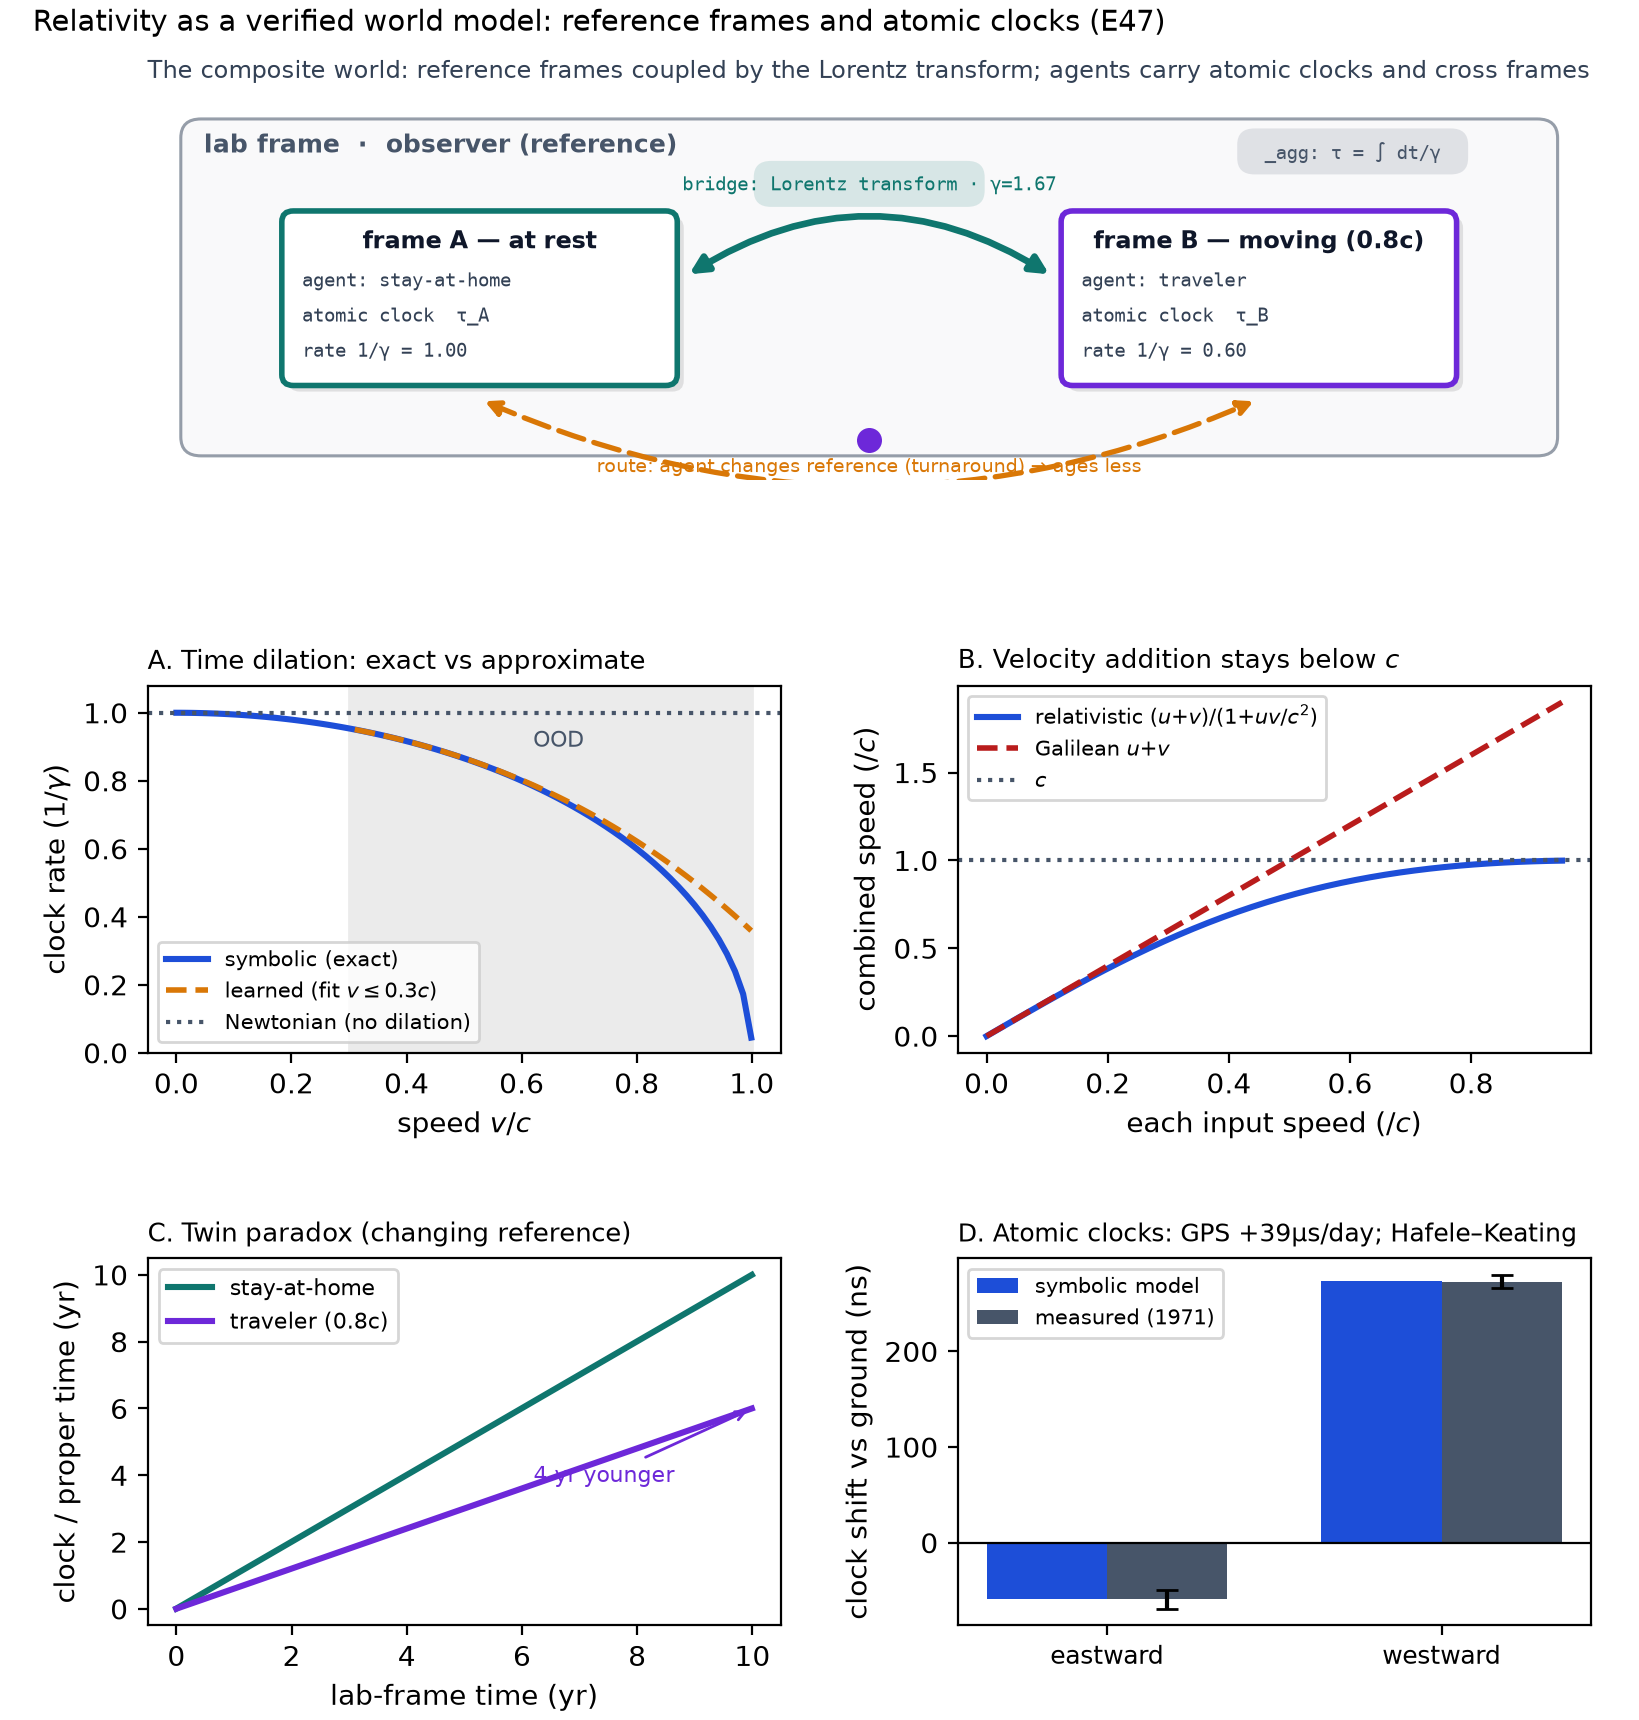
\includegraphics[width=\linewidth,height=0.48\textheight,keepaspectratio]{relativity.png}\vskip3pt{\color{owmuted}\footnotesize Twin returns 4 years younger; GPS correction +38.5 us/day from first principles\par}
\flushleft \vskip3pt{\footnotesize \begin{itemize}
  \item Time dilation exact; a low-speed learned fit diverges as v -> c
  \item Hafele--Keating east/west shifts land inside the 1971 measurements
  \item Declared, verified law where learned video models miss the physics
\end{itemize}}
\end{frame}
\begin{frame}{A same-day trading world model (E50)}
\centering
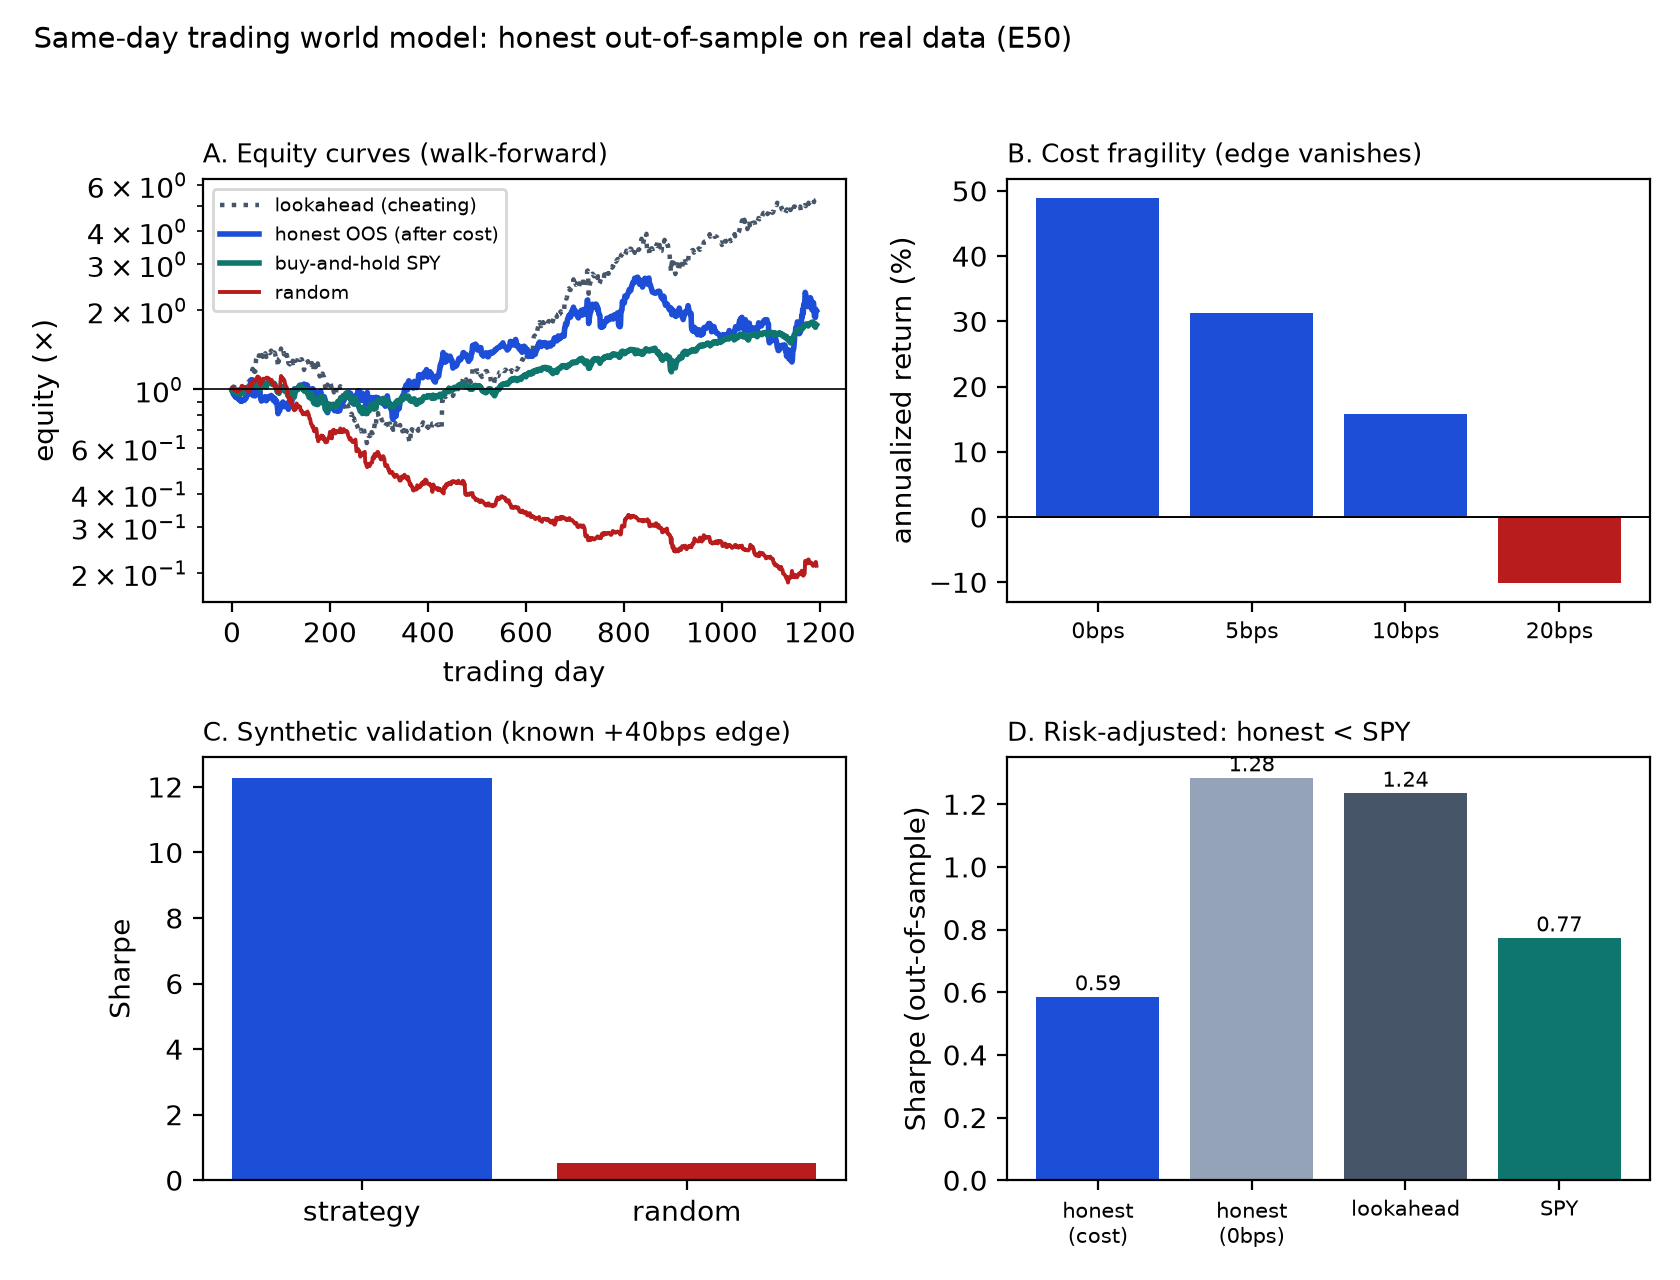
\includegraphics[width=\linewidth,height=0.48\textheight,keepaspectratio]{trading.png}\vskip3pt{\color{owmuted}\footnotesize After cost +15.7\% annualized but Sharpe 0.59 < SPY 0.77 -- honest, cost-fragile\par}
\flushleft \vskip3pt{\footnotesize \begin{itemize}
  \item Real OHLC, walk-forward, no-lookahead, after-cost backtest
  \item Recovers a known +40 bps synthetic edge, so a weak real result is real
  \item Contribution is rigor and auditability, not alpha
\end{itemize}}
\end{frame}
\begin{frame}{Wavelet denoising as perceive->world->emit (E52)}
\centering

\includegraphics[width=\linewidth,height=0.48\textheight,keepaspectratio]{denoise.png}\vskip3pt{\color{owmuted}\footnotesize Parameter-free wavelet gains +14.1 dB on edges, beating a tuned low-pass\par}
\flushleft \vskip3pt{\footnotesize \begin{itemize}
  \item Noisy signal -> sparse symbolic state (significant coefficients)
  \item Declared soft-threshold rule; inverse transform emits cleaned signal
  \item Mismatches reported: Fourier wins on smooth, Haar wrong on speech
\end{itemize}}
\end{frame}
\begin{frame}{A brain as a world-of-worlds (E58)}
\centering
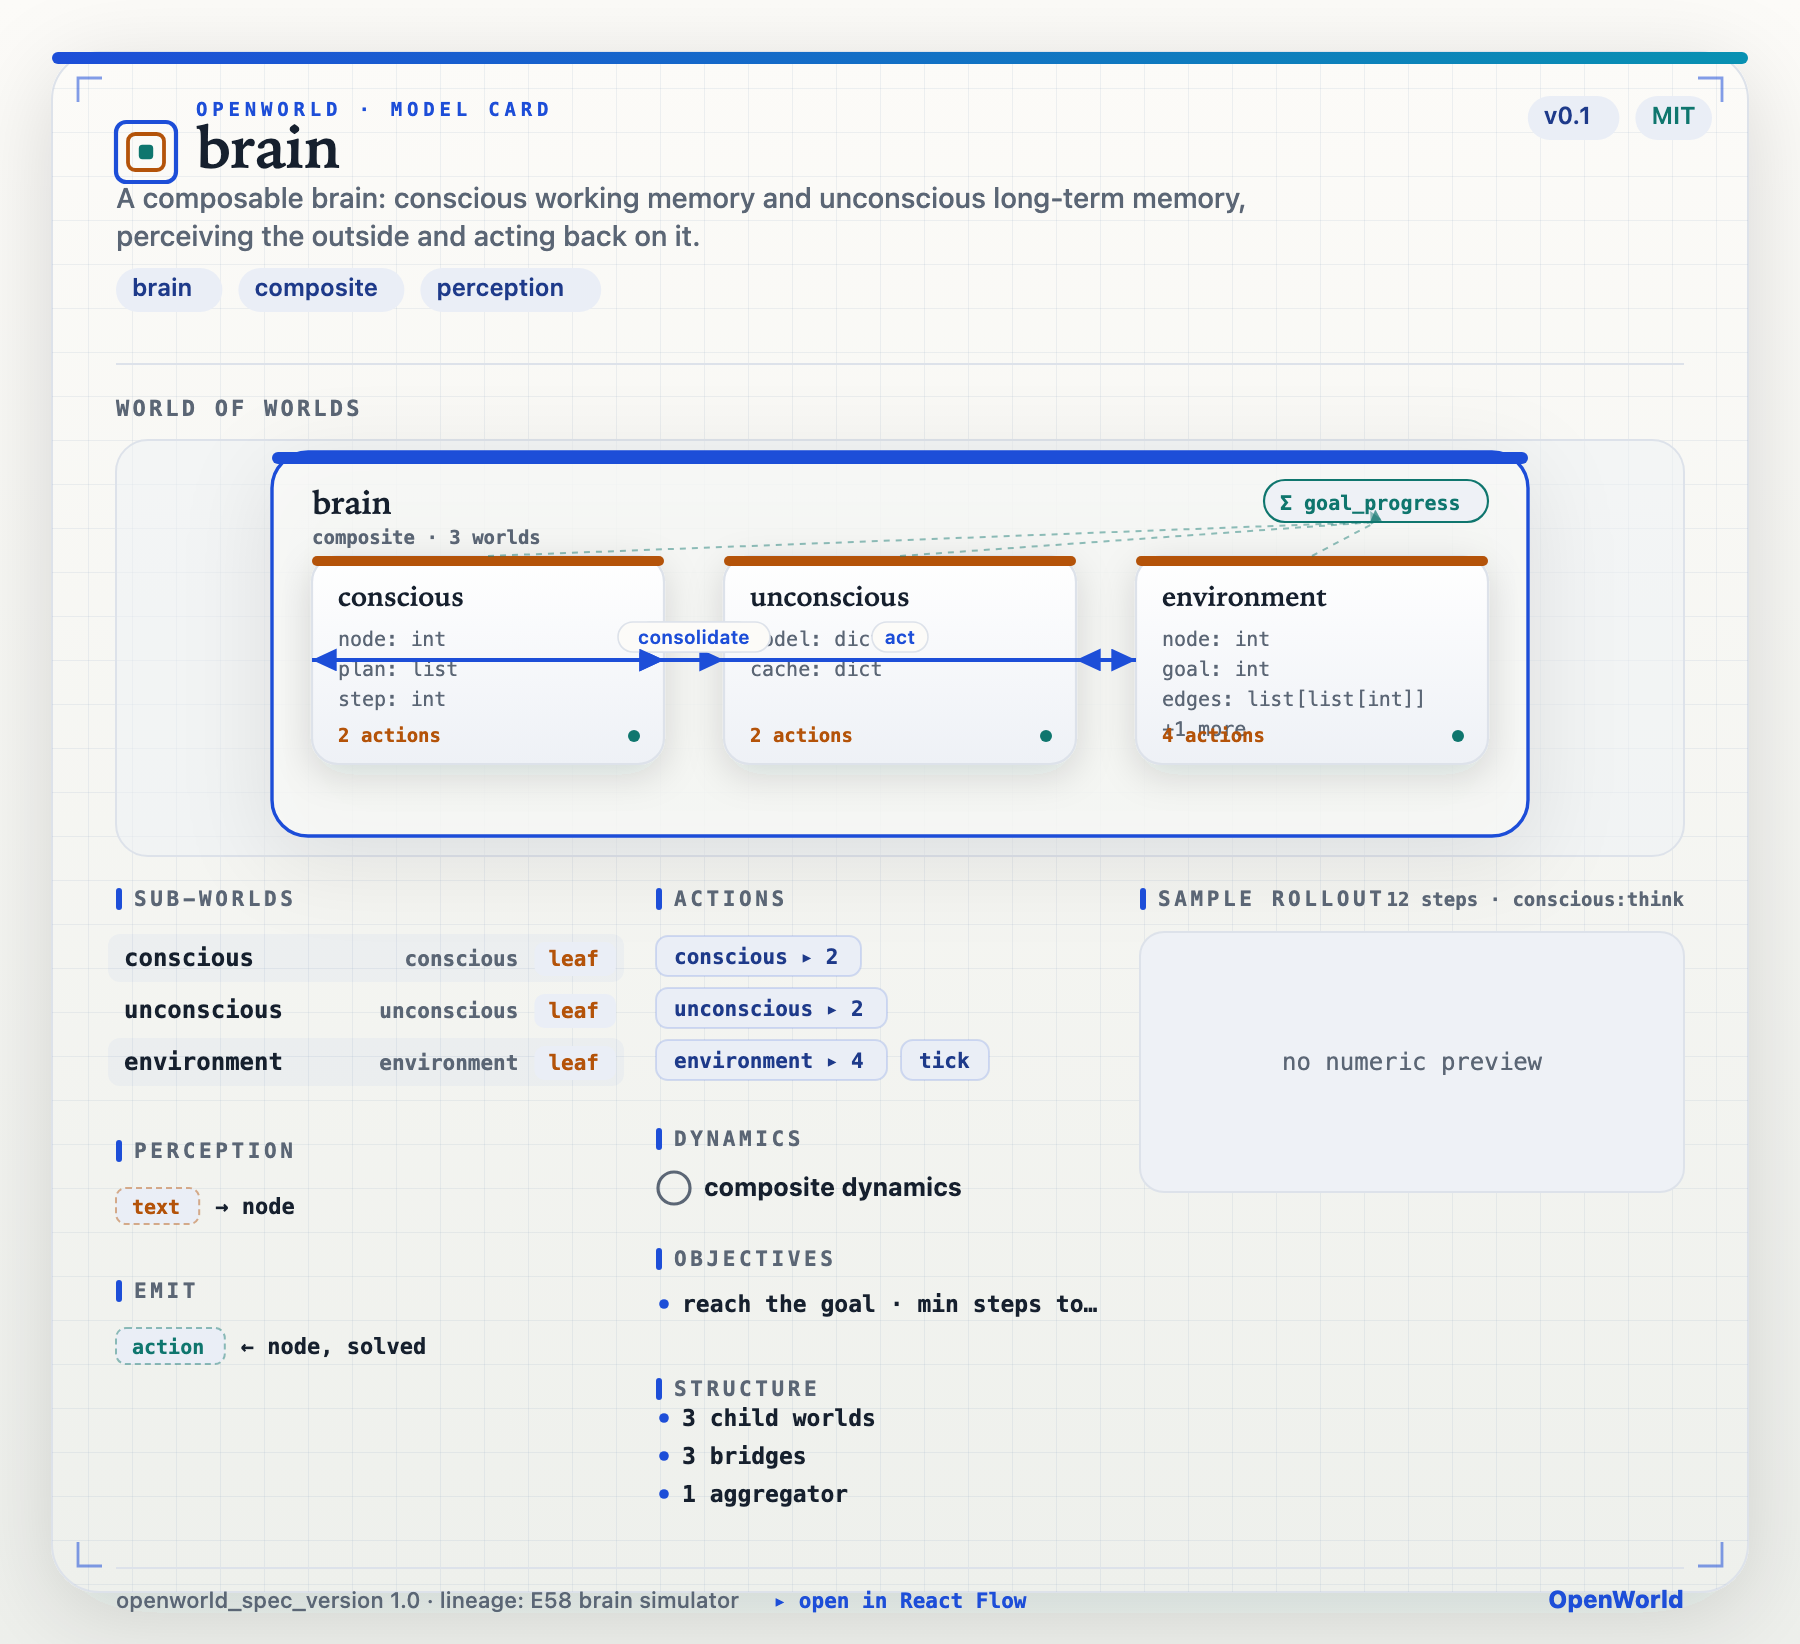
\includegraphics[width=\linewidth,height=0.48\textheight,keepaspectratio]{brain_card.png}\vskip3pt{\color{owmuted}\footnotesize Conscious + unconscious + environment, coupled by retrieve/consolidate/act bridges\par}
\flushleft \vskip3pt{\footnotesize \begin{itemize}
  \item Working memory, content-addressable long-term memory, environment
  \item Perceive -> retrieve -> think -> act -> observe -> consolidate loop
  \item The whole brain serializes to a spec and round-trips losslessly
\end{itemize}}
\end{frame}
\begin{frame}{Tree-of-thoughts ReAct with real memory (E58)}
\centering
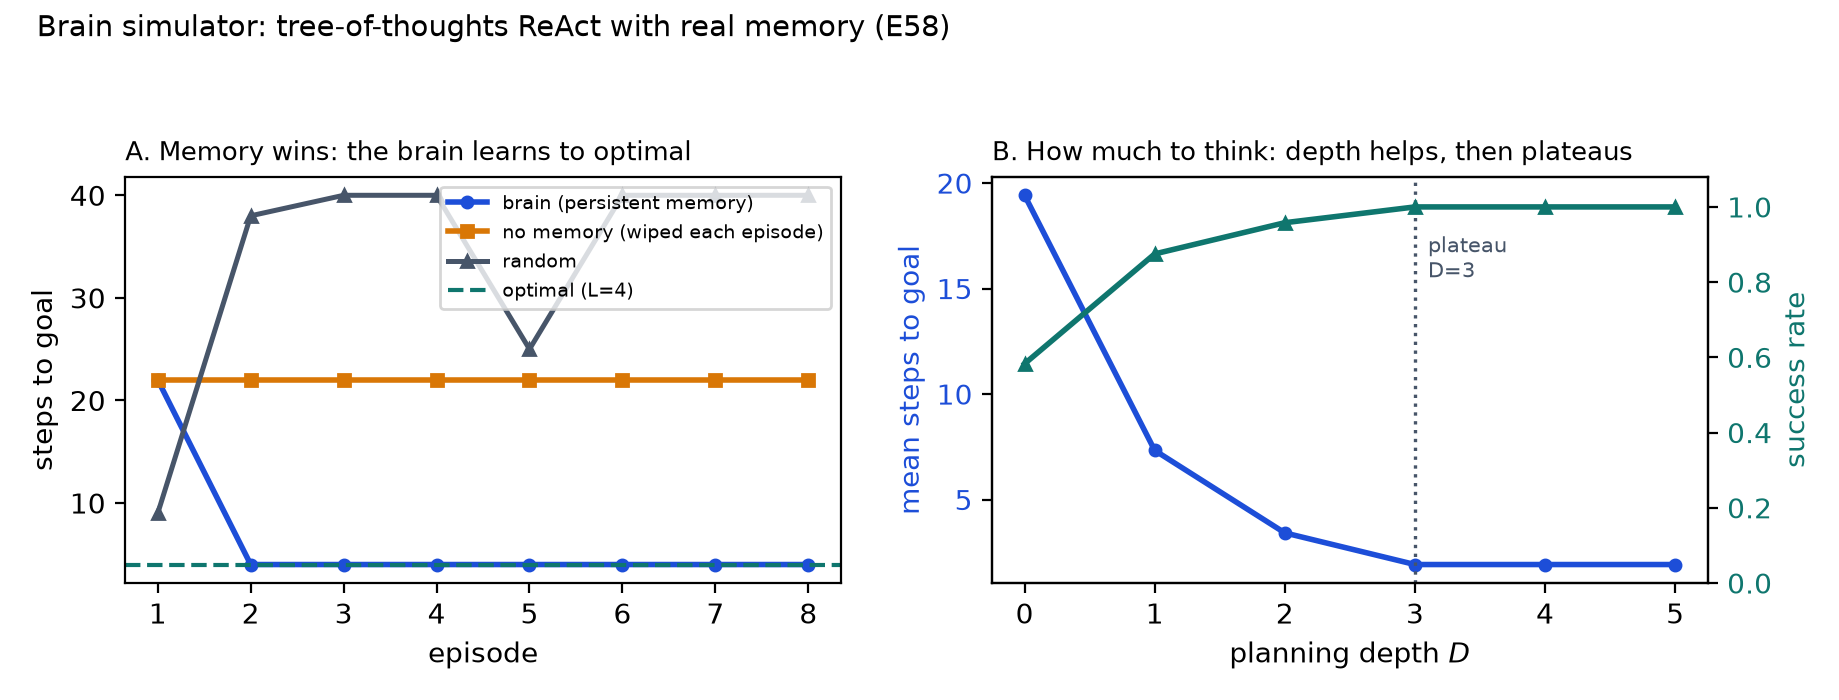
\includegraphics[width=\linewidth,height=0.48\textheight,keepaspectratio]{brain.png}\vskip3pt{\color{owmuted}\footnotesize Persistent memory reaches optimal L=4; memoryless stays \textasciitilde{}22, random flails\par}
\flushleft \vskip3pt{\footnotesize \begin{itemize}
  \item Persistent unconscious drives steps-to-goal to optimal in a couple episodes
  \item Steps fall with planning depth, plateau once depth reaches the horizon
  \item Bounded simulated lookahead helps up to the goal horizon, no further
\end{itemize}}
\end{frame}
\begin{frame}{The brain around a frozen model (E59)}
\centering
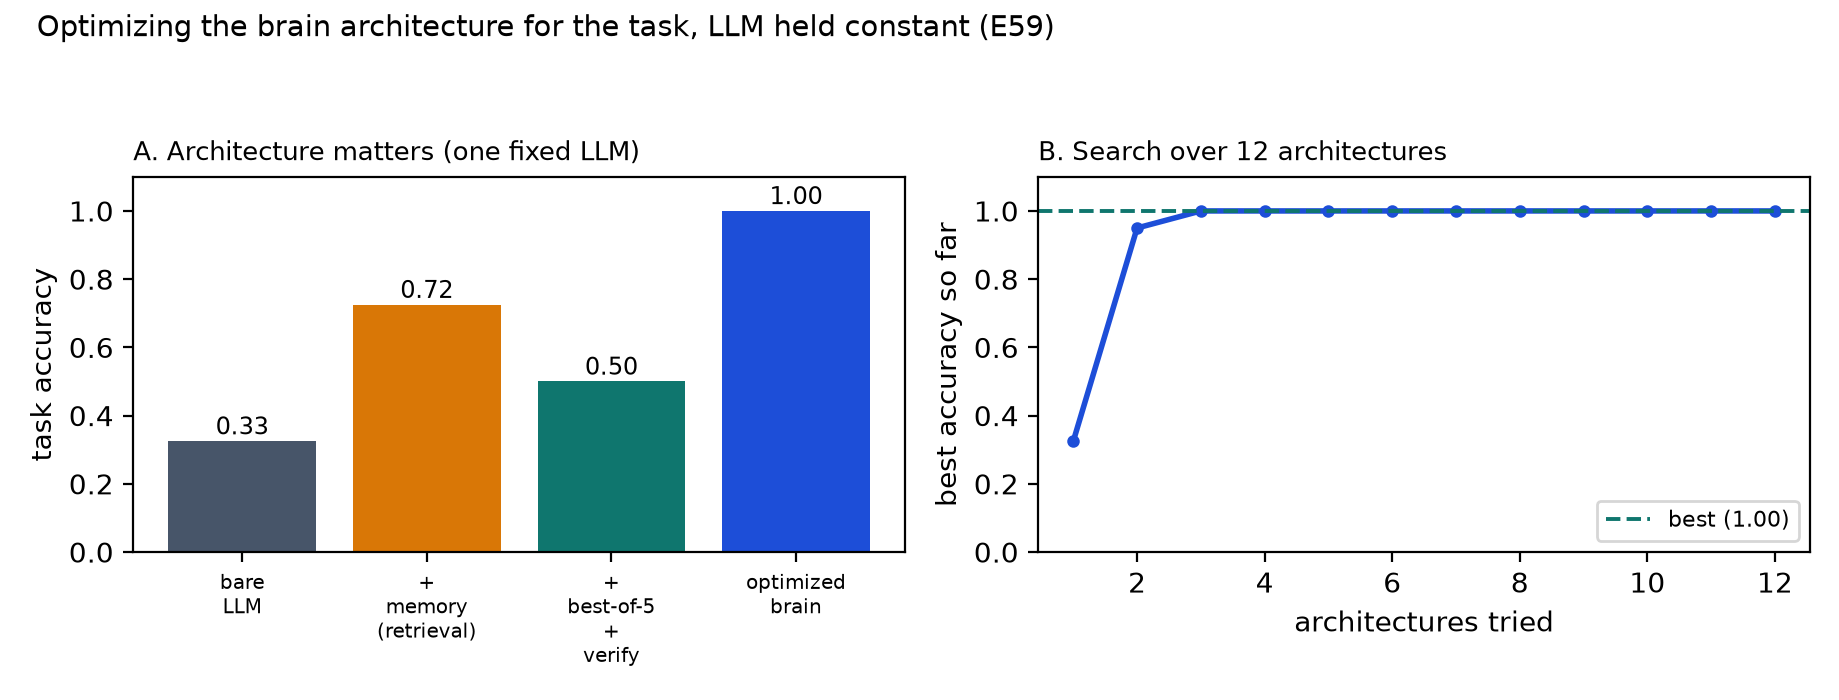
\includegraphics[width=\linewidth,height=0.48\textheight,keepaspectratio]{brain_arch.png}\vskip3pt{\color{owmuted}\footnotesize Modeled backbone: bare 0.33 -> richest brain 1.00 (+0.68), no change to the LLM\par}
\flushleft \vskip3pt{\footnotesize \begin{itemize}
  \item Retrieval makes rare-fact questions answerable; best-of-N+verify wins hard ones
  \item Ordering is a consequence of the modeling assumptions, not an empirical finding
  \item With the model frozen, the world model around it is what you optimize
\end{itemize}}
\end{frame}
\begin{frame}{The perceive->world->emit->act boundary (E60)}
\centering

\includegraphics[width=\linewidth,height=0.48\textheight,keepaspectratio]{io_boundary.png}\vskip3pt{\color{owmuted}\footnotesize Content-addressable recall routes 78\% vs Jaccard 70\% vs exact-key 0\%; resolves 78\% end to end\par}
\flushleft \vskip3pt{\footnotesize \begin{itemize}
  \item JSON/Regex perceptors + gates; MemoryStore; tool and code emitters
  \item Contract gates catch every injected malformed input and out-of-contract output
  \item All components serialize to a spec and round-trip with no LLM in the loop
\end{itemize}}
\end{frame}
\begin{frame}{Sprint allocation across a capability ladder (E35)}
\centering
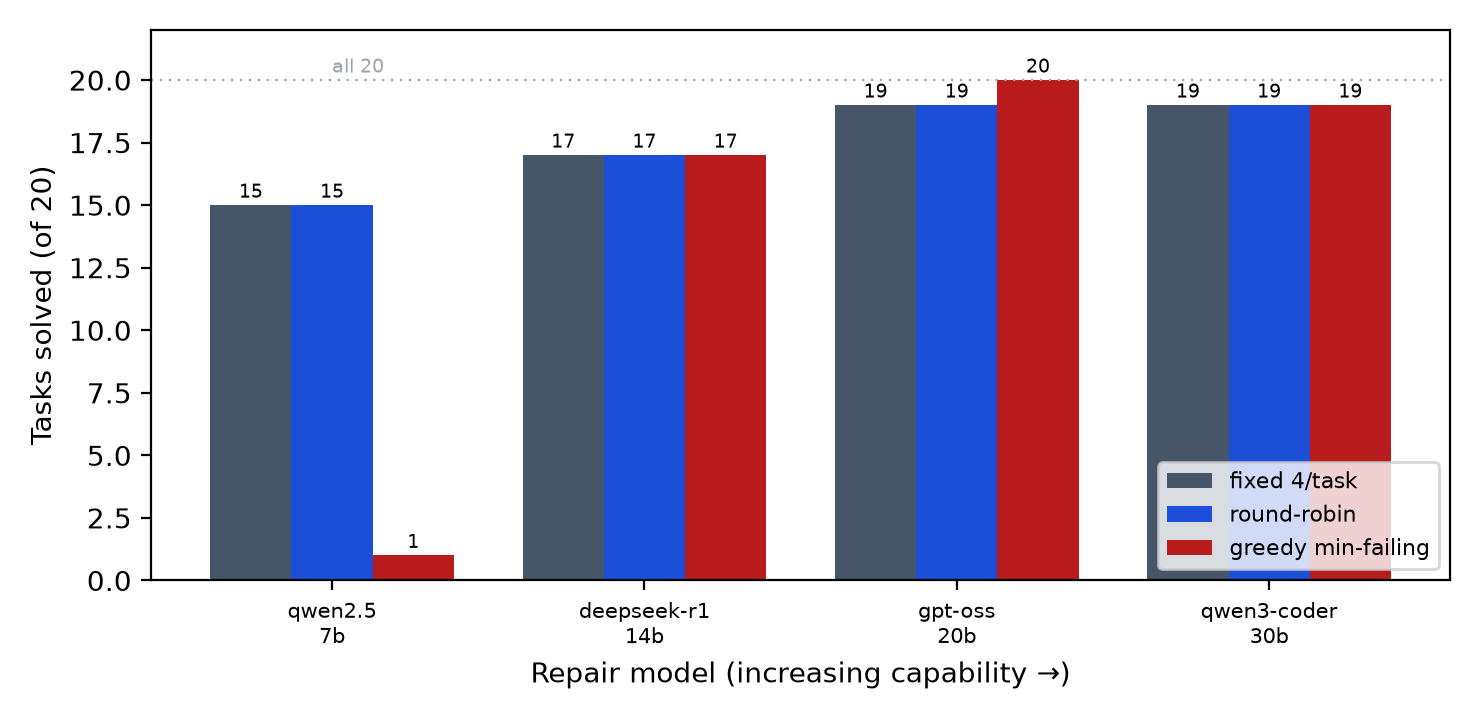
\includegraphics[width=\linewidth,height=0.48\textheight,keepaspectratio]{sprint_ladder.png}\vskip3pt{\color{owmuted}\footnotesize Fixed ceiling rises 15 -> 19/20 with capability; greedy tarpit defangs with scale\par}
\flushleft \vskip3pt{\footnotesize \begin{itemize}
  \item qwen2.5:7b -> deepseek-r1:14b -> gpt-oss:20b -> qwen3-coder:30b
  \item Greedy tarpit is capability-gated; gpt-oss:20b clears all 20
  \item Allocation policy is dominated by base model capability
\end{itemize}}
\end{frame}
\begin{frame}{Composition yields better representations (E36)}
\centering

\includegraphics[width=\linewidth,height=0.48\textheight,keepaspectratio]{representations.png}\vskip3pt{\color{owmuted}\footnotesize Every monolithic learner collapses on novel combos; the factored composite stays flat\par}
\flushleft \vskip3pt{\footnotesize \begin{itemize}
  \item Best monolith (gradient boosting) decays from 0.48 to 0.20 by K=5
  \item Collapse holds across kernels, trees, GPs, and a Koopman operator
  \item Factoring the representation -- not scaling the learner -- buys generalization
\end{itemize}}
\end{frame}
\begin{frame}{Adapting to sudden, unannounced rule changes (E41)}
\centering

\includegraphics[width=\linewidth,height=0.48\textheight,keepaspectratio]{nonstationary.png}\vskip3pt{\color{owmuted}\footnotesize Symbolic monitor re-pins the rule in 1 step; sliding-window lags, frozen never recovers\par}
\flushleft \vskip3pt{\footnotesize \begin{itemize}
  \item A reservoir's hidden regime jumps at unannounced times
  \item Explicit, identifiable program => a few observations re-pin it exactly
  \item Holds while the changed rule stays in the identifiable family
\end{itemize}}
\end{frame}
\begin{frame}{Agents traversing connected worlds with changing rules (E42)}
\centering
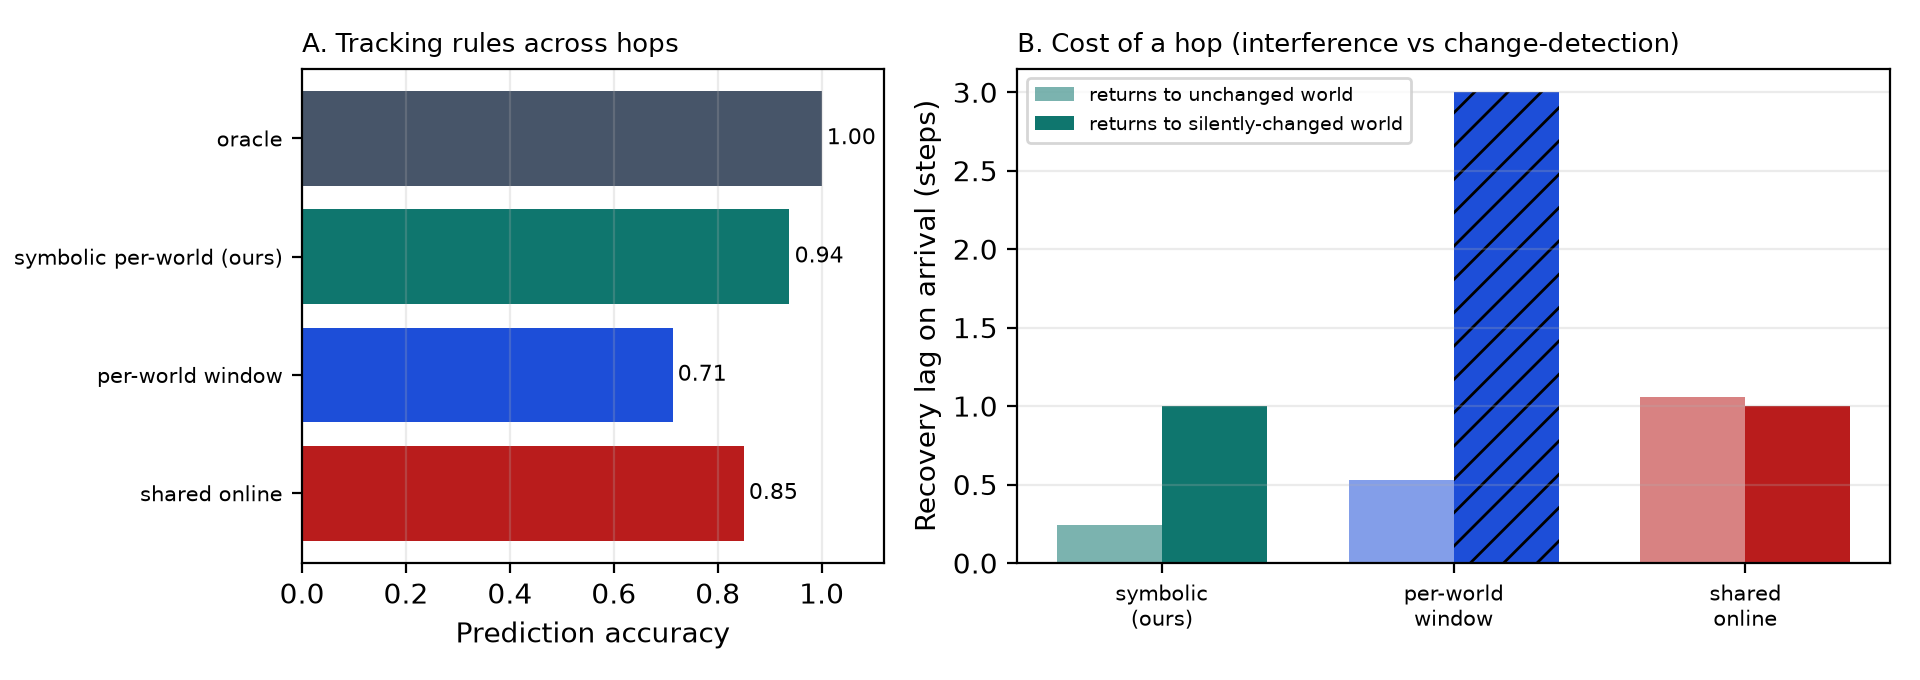
\includegraphics[width=\linewidth,height=0.48\textheight,keepaspectratio]{agent_traversal.png}\vskip3pt{\color{owmuted}\footnotesize Per-world monitor 0.94 and returns nearly free; shared learner 0.85 pays interference\par}
\flushleft \vskip3pt{\footnotesize \begin{itemize}
  \item Two non-stationary worlds joined by a toll route; agent hops between
  \item Per-world programs carry a world's rule across an absence intact
  \item A single shared belief cannot hold two worlds at once
\end{itemize}}
\end{frame}
\begin{frame}{Next-token world models: exact length generalization (E45)}
\centering
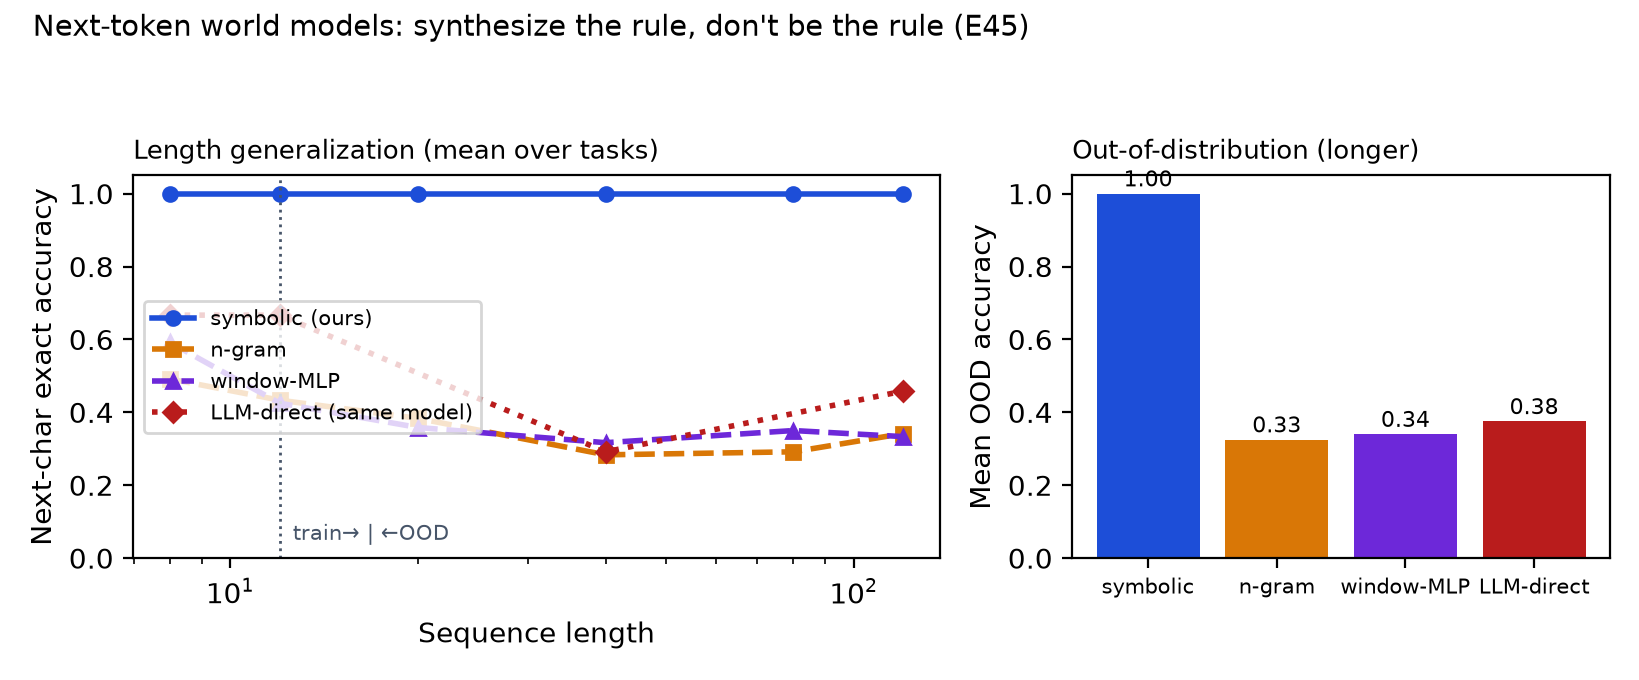
\includegraphics[width=\linewidth,height=0.48\textheight,keepaspectratio]{next_token.png}\vskip3pt{\color{owmuted}\footnotesize Induced program exact OOD on 3/3 tasks (1.00); same 30B predicting directly falls to 0.38\par}
\flushleft \vskip3pt{\footnotesize \begin{itemize}
  \item Parity, dyck, copy: memory a fixed window cannot hold
  \item Synthesize-a-program mode is length-invariant by construction
  \item n-gram and fixed-window MLP both decay with length
\end{itemize}}
\end{frame}
\begin{frame}{A database for many worlds (E46)}
\centering

\includegraphics[width=\linewidth,height=0.48\textheight,keepaspectratio]{many_worlds.png}\vskip3pt{\color{owmuted}\footnotesize Exact version space over 1e18 worlds in 191 ms; \#P boundary surfaced, not hidden\par}
\flushleft \vskip3pt{\footnotesize \begin{itemize}
  \item Likelihood factorizes over observables -> one small factor per mechanism
  \item Pluggable semiring answers Boolean, counting, and probability queries
  \item Couple w parameters non-separably and the factor grows as d\textasciicircum{}w
\end{itemize}}
\end{frame}
\begin{frame}{Path integrals over learning trajectories (E49)}
\centering

\includegraphics[width=\linewidth,height=0.48\textheight,keepaspectratio]{path_integral.png}\vskip3pt{\color{owmuted}\footnotesize Least-action curriculum reuses mastered sub-worlds -- a 6.0x speedup over from-scratch\par}
\flushleft \vskip3pt{\footnotesize \begin{itemize}
  \item Trajectory weighted by e\textasciicircum{}(-beta S); reuse the E46 semiring engine
  \item Combinatorially many trajectories summed by DP without enumeration
  \item Different starting roles (SWE, director, CEO) get different optimal paths
\end{itemize}}
\end{frame}
\begin{frame}{Abstract interpretation: sound, tight bounds (E54)}
\centering
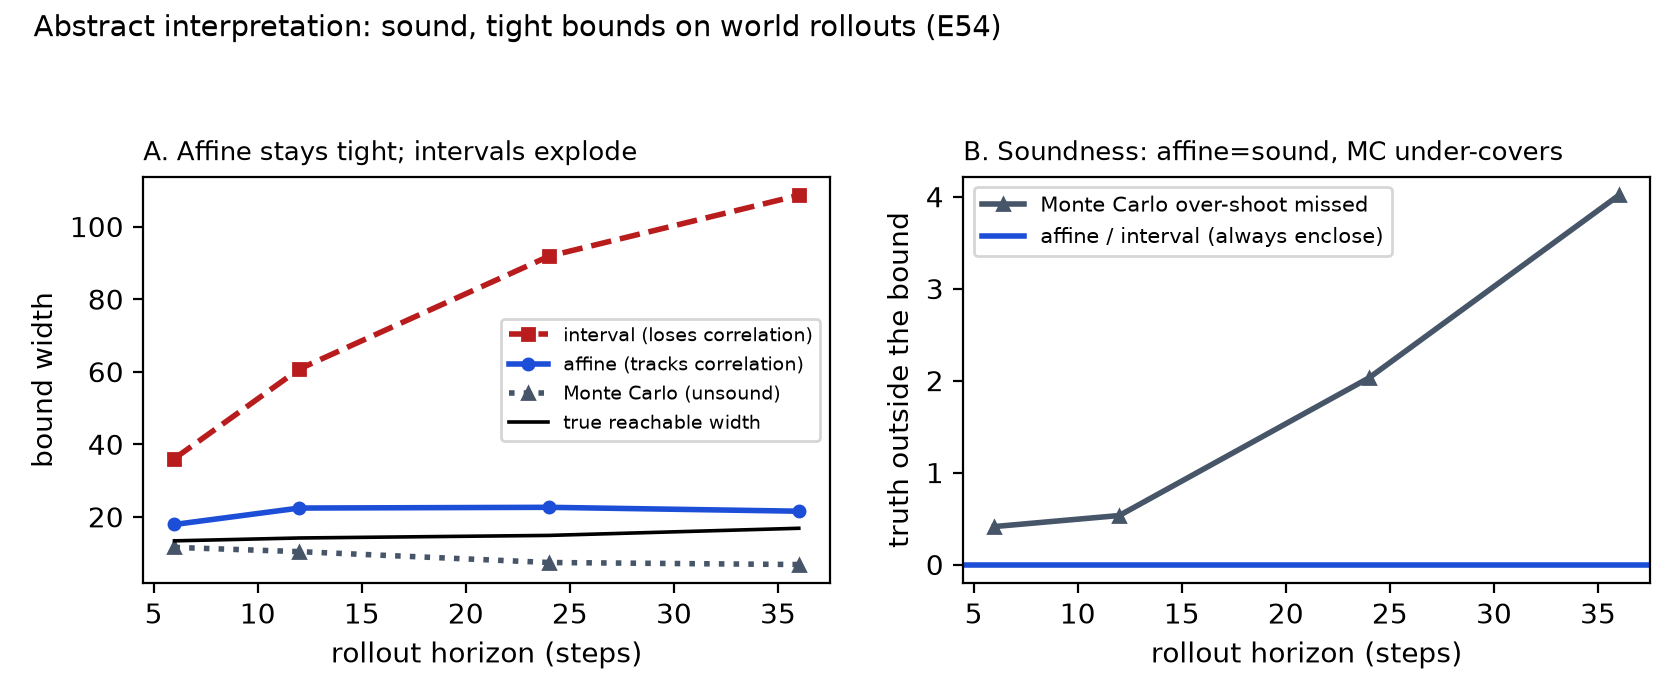
\includegraphics[width=\linewidth,height=0.48\textheight,keepaspectratio]{bounds.png}\vskip3pt{\color{owmuted}\footnotesize Affine bound width 21.5 vs interval 108.6; Monte Carlo tight but unsound\par}
\flushleft \vskip3pt{\footnotesize \begin{itemize}
  \item Run the world on abstract states -- propagate whole sets forward
  \item Affine domain tracks a/(1-a) cancellation; intervals explode
  \item Gives the world model a worst-case rollout it can certify
\end{itemize}}
\end{frame}
\begin{frame}{Information geometry: identify the world (E55)}
\centering
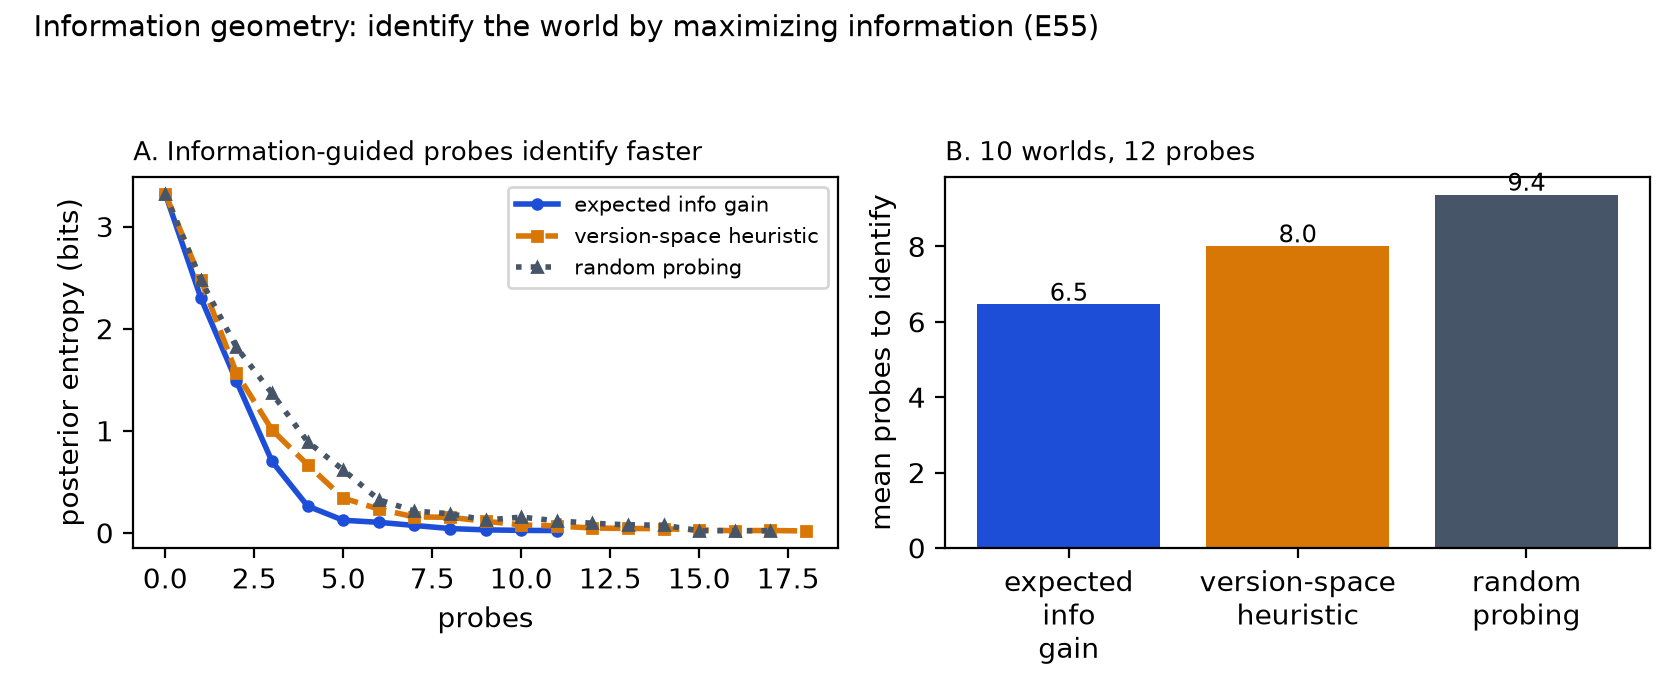
\includegraphics[width=\linewidth,height=0.48\textheight,keepaspectratio]{infogeom.png}\vskip3pt{\color{owmuted}\footnotesize Expected info gain identifies the true world in 6.5 probes vs random 9.4 (of 10 worlds)\par}
\flushleft \vskip3pt{\footnotesize \begin{itemize}
  \item Choose the probe whose outcome carries the most information
  \item Adaptivity: stop re-confirming, separate worlds still in contention
  \item Exact enumerable candidates make identification principled experiment design
\end{itemize}}
\end{frame}
\begin{frame}[plain]\vfill\centering \resizebox{0.95\textwidth}{!}{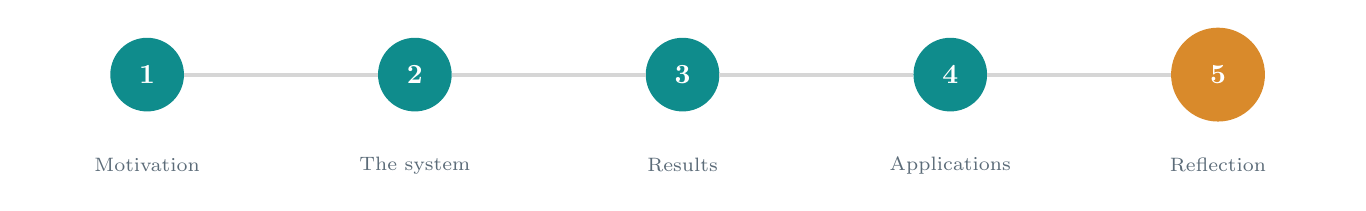
\begin{tikzpicture}[stn/.style={circle,draw=owteal,line width=1pt,minimum size=9mm,font=\bfseries,inner sep=0,text=owteal},std/.style={circle,draw=owteal,fill=owteal,line width=1pt,minimum size=9mm,font=\bfseries,inner sep=0,text=white},stc/.style={circle,draw=owochre,fill=owochre,line width=1.2pt,minimum size=11.5mm,font=\bfseries,inner sep=0,text=white},stx/.style={circle,draw=owmuted,line width=1pt,minimum size=9mm,font=\bfseries,inner sep=0,text=owmuted},stlbl/.style={font=\scriptsize,text=owmuted,align=center,text width=28mm},stln/.style={draw=black!16,line width=1.4pt}]\node[std] (s0) at (0.0,0) {1};\node[std] (s1) at (3.4,0) {2};\node[std] (s2) at (6.8,0) {3};\node[std] (s3) at (10.2,0) {4};\node[stc] (s4) at (13.6,0) {5};\node[stlbl] at (0.0,-1.15) {Motivation};\node[stlbl] at (3.4,-1.15) {The system};\node[stlbl] at (6.8,-1.15) {Results};\node[stlbl] at (10.2,-1.15) {Applications};\node[stlbl] at (13.6,-1.15) {Reflection};\draw[stln] (s0)--(s1);\draw[stln] (s1)--(s2);\draw[stln] (s2)--(s3);\draw[stln] (s3)--(s4);\end{tikzpicture}}\\[24pt]
{\color{owochre}\bfseries\footnotesize PART 5}\\[5pt]
{\color{owdeep}\bfseries\Large Reflection}\\[10pt]{\color{owmuted}\large Discussion, limitations, what comes next}\vfill\end{frame}
\begin{frame}{Interpretation: a structural trade}
\begin{itemize}
  \item Learned models buy pixel breadth, pay in compounding error and opacity
  \item Verified code buys exactness, speed, OOD transfer, auditability
  \item Within the symbolic boundary the results are one-sided
  \item The workflow: declare, verify with invariants, probe intent, tighten, recompile
  \item The artifact stays a diffable program at every stage
\end{itemize}
\end{frame}
\begin{frame}{What these worlds enable: world-time compute}
\begin{itemize}
  \item Verified worlds label trajectories exactly, for free
  \item Fine-tuning on many worlds of a domain lifts generalization to held-out worlds
  \item This is world-time compute -- the subject of the companion paper
  \item Exact, composable worlds are what make it possible
  \item But a world computer is useful whether or not one ever fine-tunes
\end{itemize}
\end{frame}
\begin{frame}{Value alignment as open specification}
\begin{itemize}
  \item Objectives are declared artifacts -- the welfare--fairness frontier is operational
  \item A weighted sum is one ethical theory (act consequentialism)
  \item Aggregators, side-constraint vetoes, and a moral parliament are distinct objects
  \item Vetoes cannot be simulated by weights (E25)
  \item Open spec manages the specification trap procedurally, does not resolve it
\end{itemize}
\end{frame}
\begin{frame}{Limitations}
\begin{itemize}
  \item Scope: symbolic-state worlds only; pixel-native remains learned territory
  \item Complexity: monolithic 7B synthesis unreliable past \textasciitilde{}8 interacting rules
  \item Scale: 20 repair tasks, 3 handwritten worlds; judges Qwen-only
  \item Judge margin is marginal (\textasciitilde{}4x cost); ensemble self-check is a screen, not a proof
  \item serve is a trusted-spec local endpoint -- no auth, sandbox is best-effort
\end{itemize}
\end{frame}
\begin{frame}{Frozen perceptual features don't control cartpole (E67)}
\begin{itemize}
  \item The perceptual species' best shot on cartpole still scores 0\%
  \item Five ways to bolt a controller onto frozen V-JEPA-2/DINOv2 all score 0
  \item Yet a probe recovers the state: R2(sin theta) = 0.95
  \item Strong frozen features are necessary but not sufficient for control
  \item End-to-end task training, not better perception, closes the gap
\end{itemize}
\end{frame}
\begin{frame}[plain]\centering\vfill
{\color{owochre}\rule{40pt}{2.5pt}}\par\vskip10pt
{\color{owdeep}\bfseries\Large Conclusion\par}\vfill\end{frame}
\begin{frame}[plain]\centering\vfill
{\color{owdeep}\bfseries\LARGE Make the model a program, verify the program, and keep the values dialable -- an orthogonal path to scaling parameters until hallucination is suppressed.\par}\vfill\end{frame}
\begin{frame}{Takeaways and next steps}
\begin{itemize}
  \item A training-free symbolic world model is bit-exact where learned dynamics compound error
  \item Composition defeats the complexity cliff; the boundary is measured, not hidden
  \item 100 worlds in minutes on a laptop; portable, auditable, shareable specs
  \item Next: compositional synthesis, standard-scale coding, hybrid perception-to-symbol
  \item All code, 100 recipes, and 79 experiments regenerate from one repository
\end{itemize}
\end{frame}
\end{document}
